% =====================================================================
% Rapport de stage --- RCA microservices : pipeline GNN reproductible et deployable
% Wassim Badraoui, EPITA / Devoteam, 2026
% =====================================================================
\documentclass[a4paper,11pt,oneside]{report}

% --- Encoding / fonts / language ---------------------------------------
\usepackage[utf8]{inputenc}
\usepackage[T1]{fontenc}
\usepackage{lmodern}
\usepackage[french]{babel}
\frenchsetup{SmallCapsFigTabCaptions=false,AutoSpacePunctuation=false}

% --- Geometry, headers, line spacing ----------------------------------
\usepackage[a4paper,margin=2.5cm]{geometry}
\usepackage{setspace}
\setstretch{1.15}
\usepackage{fancyhdr}
\pagestyle{fancy}
\fancyhf{}
\fancyhead[L]{\nouppercase{\leftmark}}
\fancyhead[R]{\thepage}
\renewcommand{\headrulewidth}{0.4pt}

% --- Math --------------------------------------------------------------
\usepackage{amsmath,amssymb,amsthm,mathtools}

% --- Tables ------------------------------------------------------------
\usepackage{booktabs,array,longtable,tabularx}
\usepackage{multirow}

% --- Figures / colors / TikZ ------------------------------------------
\usepackage{graphicx}
\usepackage[dvipsnames,table]{xcolor}
\usepackage{caption}
\usepackage{subcaption}
\usepackage{tikz}
\usetikzlibrary{positioning,arrows.meta,calc,fit,shapes.geometric}

% --- Code listings -----------------------------------------------------
\usepackage{listings}
\definecolor{codegray}{HTML}{F4F4F4}
\definecolor{codekeyword}{HTML}{0F62FE}
\definecolor{codestring}{HTML}{198038}
\definecolor{codecomment}{HTML}{8D8D8D}
\lstdefinestyle{base}{
  backgroundcolor=\color{codegray},
  basicstyle=\ttfamily\footnotesize,
  keywordstyle=\color{codekeyword}\bfseries,
  stringstyle=\color{codestring},
  commentstyle=\color{codecomment}\itshape,
  numbers=none,
  frame=single,
  framesep=4pt,
  rulecolor=\color{black!10},
  breaklines=true,
  breakatwhitespace=true,
  showstringspaces=false,
  tabsize=2,
  captionpos=b,
}
\lstdefinestyle{python}{style=base,language=Python}
\lstdefinestyle{yaml}{style=base,morekeywords={apiVersion,kind,metadata,spec,template,containers,resources,env},keywordstyle=\color{codekeyword}\bfseries}
\lstdefinestyle{shell}{style=base,language=bash}

% --- Bibliography ------------------------------------------------------
\usepackage[backend=biber,style=numeric-comp,sorting=nyt,maxbibnames=99]{biblatex}
\addbibresource{bibliography.bib}

% --- Hyperlinks --------------------------------------------------------
\usepackage[hidelinks]{hyperref}
\hypersetup{
  pdftitle={Root Cause Analysis pour microservices --- Pipeline GNN reproductible et deployable},
  pdfauthor={Wassim Badraoui},
  pdfsubject={Rapport de stage --- RCA / GNN / Kubernetes},
  pdfkeywords={RCA, GNN, microservices, Kubernetes, Optuna, FastAPI},
  colorlinks=false,
  linktoc=all,
}
\usepackage[capitalise]{cleveref}
% --- Cleveref noms en francais ----------------------------------------
\crefname{chapter}{chapitre}{chapitres}
\Crefname{chapter}{Chapitre}{Chapitres}
\crefname{section}{section}{sections}
\Crefname{section}{Section}{Sections}
\crefname{subsection}{section}{sections}
\Crefname{subsection}{Section}{Sections}
\crefname{table}{table}{tables}
\Crefname{table}{Table}{Tables}
\crefname{figure}{figure}{figures}
\Crefname{figure}{Figure}{Figures}
\crefname{equation}{\'equation}{\'equations}
\Crefname{equation}{\'Equation}{\'Equations}

% --- Header titre des chapitres reduit --------------------------------
\usepackage{titlesec}
\titleformat{\chapter}[display]
  {\normalfont\huge\bfseries}{Chapitre \thechapter}{18pt}{\LARGE}
\titlespacing*{\chapter}{0pt}{0pt}{20pt}

% =====================================================================
% Document
% =====================================================================
\begin{document}

% -----------------------------------------------------------------------
% Page de garde
% -----------------------------------------------------------------------
\begin{titlepage}
  \centering
  \vspace*{1cm}
  {\Large\bfseries EPITA \par}
  {\large \'Ecole d'Ing\'enieurs en Informatique \par}
  \vspace{0.5cm}
  \rule{0.6\textwidth}{0.5pt}\par
  \vspace{0.5cm}
  {\large Stage industriel chez \textbf{Devoteam} \par}
  \vspace{3cm}
  {\Huge\bfseries Root Cause Analysis dans les architectures microservices \par}
  \vspace{0.8cm}
  {\Large\itshape Un pipeline graphe-temporel reproductible et d\'eployable, du benchmark \`a la production sur cluster Kubernetes \par}
  \vspace{3cm}
  {\Large \textbf{Wassim Badraoui} \par}
  \vspace{0.3cm}
  {\large \texttt{wassim.badraoui@epita.fr} \par}
  \vfill
  \rule{0.6\textwidth}{0.5pt}\par
  \vspace{0.5cm}
  {\large Rapport de stage --- 2026 \par}
  \vspace{0.3cm}
  {\small Tuteur entreprise (Devoteam) \quad\textbar\quad Tuteur acad\'emique (EPITA) \par}
\end{titlepage}

% -----------------------------------------------------------------------
% Remerciements
% -----------------------------------------------------------------------
\chapter*{Remerciements}
\addcontentsline{toc}{chapter}{Remerciements}

Je tiens \`a remercier mon tuteur entreprise au sein de \textbf{Devoteam} pour son accompagnement tout au long du stage, et en particulier pour l'acc\`es au cluster Kubernetes \texttt{observit-cluster1} qui a rendu possibles les exp\'eriences de collecte de t\'el\'em\'etrie et d'injection de chaos. Sans ce terrain de jeu r\'eel, le travail serait rest\'e cantonn\'e \`a des donn\'ees synth\'etiques.

Je remercie \'egalement mon tuteur acad\'emique \`a l'\textbf{EPITA} pour ses conseils m\'ethodologiques sur la mise en place du protocole exp\'erimental (s\'eparation train/test, gestion des seeds, matrice de comparabilit\'e). Ces \'echanges ont structur\'e la rigueur du protocole.

Enfin, merci aux auteurs du benchmark public \textbf{RCAEval} pour avoir rendu reproductible un volet souvent flou de la litt\'erature : les chiffres des baselines RCA. Sans cette r\'ef\'erence, m\^eme indicative, il aurait \'et\'e impossible de positionner ce travail.

% -----------------------------------------------------------------------
% Resume + Abstract
% -----------------------------------------------------------------------
\chapter*{R\'esum\'e}
\addcontentsline{toc}{chapter}{R\'esum\'e}

L'analyse de cause racine (RCA) dans les architectures microservices est une t\^ache critique et difficile~: les pannes se propagent dans le graphe de d\'ependances, les signaux observ\'es sont bruit\'es, et l'espace de recherche cro\^it avec le nombre de services instrument\'es. Ce stage pr\'esente STA (\emph{Select-Then-Analyze}), un r\'eseau de neurones spatio-temporel \`a goulot d'\'etranglement pr\'ecoce qui r\'eduit la complexit\'e du RCA de $O(N^2)$ \`a $O(N + k^2)$ en s\'electionnant un sous-graphe candidat compact avant l'analyse spatiale profonde. STA combine un encodeur temporel local, un s\'electeur diff\'erentiable \`a estimateur \emph{Straight-Through}, et une r\'egularisation \emph{Variational Graph Information Bottleneck}.

Quatre variantes du mod\`ele (STA, GATv2, STA-MM, GATv2-MM) sont \'evalu\'ees sur quatre r\'egimes exp\'erimentaux~: graphes synth\'etiques Barab\'asi-Albert ($N \in \{20,50,100\}$), trois jeux de donn\'ees publics RCAEval ($N{=}5$), un cluster Kubernetes priv\'e ex\'ecutant sock-shop ($N{=}14$), et un d\'eploiement microservices synth\'etique-mais-r\'eel \`a $N{=}50$ sur ce m\^eme cluster. Trois r\'esultats principaux~:
\begin{enumerate}
  \item L'avantage de complexit\'e de STA est r\'eel mais \emph{modeste et coh\'erent en direction} \`a $N \ge 50$~: $+6{,}3$~pp Avg@1 vs.\ GATv2 \`a $N{=}100$ \`a 5 seeds (ramen\'e \`a $+2{,}4$~pp \`a 10 seeds, cf.\ \cref{sec:robustesse}), et $+5{,}8$~pp \`a $N{=}50$ sur le cluster. Je ne revendique aucun SOTA~; une r\'eimpl\'ementation isop\'erim\`etre de BARO (\cref{tab:baro-iso}) le bat m\^eme sur \texttt{online-boutique}.
  \item \`A petite \'echelle ($N \le 14$), STA et GATv2 sont \emph{dans le bruit} d'une \'evaluation \`a 5 seeds.
  \item La fusion multimodale (m\'etriques + logs + traces) d\'egrade les performances sur RCAEval ($-5\,\%$ Avg@1 sur trainticket) mais ne r\'egresse pas sur le cluster priv\'e --- la qualit\'e des modalit\'es auxiliaires est un facteur confondant probable.
\end{enumerate}

Au-del\`a de l'\'evaluation, j'ai mis en place une cha\^ine op\'erationnelle compl\`ete~: optimisation automatique des hyperparam\`etres par Optuna (25 essais TPE), persistance d'un \emph{bundle} portable mod\`ele + scaler + m\'etadonn\'ees + tra\c{c}abilit\'e HPO, conteneurisation, et d\'eploiement effectif comme service FastAPI sur le cluster Devoteam avec int\'egration Prometheus. Le manuscrit \texttt{PAPER.md}, les artefacts JSON canoniques (SHA-256), le code source et les manifestes Kubernetes sont publi\'es \`a \url{https://github.com/Wassbdr/matrix_simple}.

\vspace{0.5cm}
\textbf{Mots-cl\'es}~: Root Cause Analysis, microservices, r\'eseaux de neurones spatio-temporels, Information Bottleneck, Kubernetes, Chaos Mesh, Optuna, FastAPI.

\chapter*{Abstract (English)}
\addcontentsline{toc}{chapter}{Abstract (English)}

Root Cause Analysis (RCA) in microservice architectures is challenging because failures propagate across service dependency graphs, observable signals are noisy, and the search space grows with the number of instrumented services. This work presents STA (Select-Then-Analyze), an early-bottleneck spatio-temporal graph neural network that reduces RCA complexity from $O(N^2)$ to $O(N + k^2)$ by selecting a compact candidate subgraph before deep spatial analysis. STA combines a zero-hop temporal encoder, a differentiable Straight-Through Estimator selector, and Variational Graph Information Bottleneck regularization.

Four model variants (STA, GATv2, STA-MM, GATv2-MM) are evaluated across four regimes: synthetic Barab\'asi-Albert graphs ($N \in \{20,50,100\}$), three public RCAEval datasets ($N{=}5$), a private Kubernetes cluster running sock-shop ($N{=}14$), and a 50-service synthetic-but-real deployment on the same cluster. This is a deliberately honest study, not a SOTA claim. Four findings: (i) STA's $O(N+k^2)$ design keeps per-query latency flat as $N$ grows, and its accuracy edge is real but modest and shrinks under scrutiny ($+6.2 \to +2.3$~pp Avg@1 at $N{=}100$ from 5 to 10 seeds; $+5.7$~pp on the $N{=}50$ cluster); (ii) at small graph scale ($N \le 14$), STA, GATv2 and a strong statistical baseline are within noise; (iii) an isoperimetric re-run of BARO (same cases/split/metrics) shows it is far stronger than its published number and beats my models on Online Boutique --- no SOTA claim; (iv) multimodal fusion degrades or matches metrics-only on RCAEval while halving variance on the cluster, a consistent negative result. Beyond evaluation, the project delivers an end-to-end operational pipeline: Optuna hyperparameter optimization, a persisted model bundle, a containerized FastAPI inference service, and a live Kubernetes deployment with Prometheus integration.

\vspace{0.5cm}
\textbf{Keywords}: Root Cause Analysis, microservices, spatio-temporal GNN, Information Bottleneck, Kubernetes, Chaos Mesh, Optuna, FastAPI.

% -----------------------------------------------------------------------
% Tables
% -----------------------------------------------------------------------
\tableofcontents
\listoffigures
\listoftables

\cleardoublepage
\pagenumbering{arabic}

% =====================================================================
% Chapitre 1 --- Introduction
% =====================================================================
\chapter{Introduction}
\label{chap:introduction}

\section{Contexte industriel}
\label{sec:contexte}

Les applications natives du cloud d\'eploient leur logique m\'etier sur quelques dizaines \`a quelques centaines de microservices faiblement coupl\'es. Cette architecture apporte des b\'en\'efices clairs --- d\'eploiements ind\'ependants, mise \`a l'\'echelle horizontale par composant, isolation des d\'efaillances --- mais transforme la pratique de l'op\'eration en un probl\`eme d'observabilit\'e distribu\'ee. Lorsqu'un incident survient, identifier le service \`a l'origine de la d\'efaillance (la \emph{cause racine}) parmi $N$ services est un pr\'erequis \`a toute rem\'ediation automatis\'ee. Dans les environnements de production comportant plusieurs dizaines de services instrument\'es, le temps moyen d'identification d'une cause racine par triage manuel atteint r\'eguli\`erement plusieurs dizaines de minutes, avec un impact \'economique direct.

\section{Difficult\'es structurelles du RCA microservices}
\label{sec:difficultes}

Le RCA pour microservices est difficile pour trois raisons li\'ees~:

\begin{itemize}
  \item \textbf{Les pannes se propagent.} Un service d\'efectueux \'emet des erreurs et des latences anormales vers ses appelants, qui les propagent en cascade --- le sympt\^ome le plus visible n'est presque jamais la cause.
  \item \textbf{Les signaux sont h\'et\'erog\`enes.} L'observabilit\'e moderne couvre les m\'etriques (CPU, m\'emoire, latence, taux d'erreur), les logs (\'ev\'enements discrets, codes d'erreur) et les traces (chemins de requ\^ete bout-en-bout). Chaque modalit\'e capte une facette du diagnostic et peut compl\'eter ou contredire les autres.
  \item \textbf{L'espace de recherche cro\^it.} Une analyse spatiale na\"ive co\^ute $O(N^2)$ op\'erations \`a la couche de convolution graphe~; \`a $N{=}500$, ce co\^ut devient prohibitif pour un diagnostic en temps r\'eel.
\end{itemize}

\section{Questions de recherche du stage}
\label{sec:questions}

Plusieurs questions restent peu trait\'ees par la litt\'erature publique~:

\begin{enumerate}
  \item \textbf{Scalabilit\'e.} Le goulot d'\'etranglement spatial des GNN \emph{full-graph} limite-t-il leur d\'eploiement \`a grand $N$, et un \'etage de s\'election principi\'e r\'eduit-il ce co\^ut sans sacrifier le rappel~?
  \item \textbf{Graphe vs.\ temporel.} \`A l'\'echelle des benchmarks publics (typiquement $N{=}5$), incorporer la structure graphe am\'eliore-t-il vraiment l'identification de la cause racine, ou ajoute-t-il du bruit~?
  \item \textbf{Int\'egration multimodale.} Les logs et les traces compl\`etent-ils les m\'etriques en pratique, ou introduisent-ils des conflits de gradients qui d\'egradent la performance globale~?
  \item \textbf{Robustesse op\'erationnelle.} Comment un mod\`ele RCA se comporte-t-il pendant les transitions de d\'eploiement Kubernetes (\emph{concept drift}) et face aux \emph{gray failures}, ces anomalies qui restent en dessous des seuils d'alerte individuels mais d\'egradent l'exp\'erience syst\`eme~?
\end{enumerate}

\section{Contributions du stage}
\label{sec:contributions}

Ce stage apporte quatre contributions concr\`etes pour r\'epondre \`a ces questions~:

\begin{enumerate}
  \item \textbf{STA (Select-Then-Analyze)} (\cref{chap:methode})~: un GNN \`a goulot d'\'etranglement pr\'ecoce qui atteint une complexit\'e $O(N + k^2)$ via une s\'election top-$k$ diff\'erentiable r\'egularis\'ee par GIB variationnel. STA permet une analyse spatio-temporelle profonde sur un sous-graphe candidat compact tout en conservant un entra\^inement de bout en bout via un \emph{Straight-Through Estimator}~\cite{bengio2013ste,jang2017gumbel}.
  \item \textbf{\'Evaluation multi-r\'egime syst\'ematique} (\cref{chap:experiences,chap:resultats})~: quatre variantes du mod\`ele sont compar\'ees sur graphes synth\'etiques, trois jeux de donn\'ees RCAEval, le cluster Devoteam (sock-shop $N{=}14$) et un d\'eploiement \`a $N{=}50$ sur ce m\^eme cluster. Avg@$k$, MRR et NDCG@3 sont report\'es avec leurs \'ecarts-types sur 5 seeds (3 pour $N{=}50$).
  \item \textbf{R\'esultat n\'egatif robuste sur la fusion multimodale} (\cref{sec:resultats-mm})~: sur RCAEval, fusionner logs et traces avec les m\'etriques n'am\'eliore pas (et d\'egrade m\^eme parfois) les performances par rapport au mod\`ele m\'etriques seules. Le r\'esultat est document\'e avec ses caveats m\'ethodologiques et a des implications de d\'eploiement directes.
  \item \textbf{Pile op\'erationnelle compl\`ete} (\cref{chap:hpo-deploiement})~: HPO automatique par Optuna, persistance d'un \emph{bundle} portable (mod\`ele + scaler + m\'etadonn\'ees + tra\c{c}abilit\'e HPO), conteneurisation, et d\'eploiement effectif sur le cluster Devoteam comme service FastAPI avec int\'egration Prometheus. Le manuscrit accompagnant inclut aussi un d\'etecteur de drift bas\'e sur ADWIN~\cite{bifet2007adwin} et un d\'etecteur de \emph{gray failure} \`a quatre m\'ecanismes.
\end{enumerate}

\section{Organisation du m\'emoire}
\label{sec:plan}

Le rapport est structur\'e comme suit~:
\begin{itemize}
  \item \cref{chap:etat-de-lart} pr\'esente l'\'etat de l'art en RCA pour microservices, GNN spatio-temporels, GIB, diagnostic multimodal et \emph{gray failures}.
  \item \cref{chap:formulation} formalise le RCA comme un probl\`eme inverse parcimonieux et d\'efinit la taxonomie des types de pannes.
  \item \cref{chap:methode} d\'etaille les quatre architectures de mod\`ele et les composants op\'erationnels (cascade-aware loss, ADWIN drift detector, gray failure detector, causal graph builder).
  \item \cref{chap:experiences} d\'ecrit les jeux de donn\'ees, le protocole exp\'erimental et la matrice de comparabilit\'e aux baselines publi\'ees.
  \item \cref{chap:resultats} pr\'esente les r\'esultats sur quatre r\'egimes exp\'erimentaux et les ablations.
  \item \cref{chap:hpo-deploiement} d\'ecrit l'optimisation automatique des hyperparam\`etres et le d\'eploiement effectif sur le cluster Devoteam.
  \item \cref{chap:discussion} discute les forces, les limites et les implications du travail.
  \item \cref{chap:conclusion} conclut et liste les pistes futures.
  \item Les annexes regroupent la table de reproductibilit\'e, la structure du \emph{bundle}, la chronologie du stage et la matrice de comparabilit\'e.
\end{itemize}

% =====================================================================
% Chapitre 2 --- Etat de l'art
% =====================================================================
\chapter{\'Etat de l'art}
\label{chap:etat-de-lart}

\section{RCA pour microservices}
\label{sec:eda-rca}

Les premiers syst\`emes de RCA pour microservices s'appuient sur la propagation par corr\'elation~: \textbf{MicroRCA} construit un graphe de services pond\'er\'e \`a partir des corr\'elations de Pearson entre m\'etriques et applique une marche al\'eatoire pour classer les nœuds candidats~; \textbf{CausaRank} am\'eliore cette approche par une formulation de classement causal~; \textbf{E-Diagnosis} introduit un apprentissage de repr\'esentations d\'es-entrem\^el\'ees pour s\'eparer les types d'anomalies~; et \textbf{BARO} utilise un classement par bootstrap sur les m\'etriques de service, qui atteint les meilleures performances publi\'ees sur les jeux de donn\'ees RCAEval (Avg@1~$\approx$~0{,}71).

Le benchmark public \textbf{RCAEval}\footnote{\url{https://github.com/phamquiluan/RCAEval}} fournit un cadre d'\'evaluation standardis\'e couvrant trainticket, sockshop, online-boutique et d'autres applications microservices, ainsi que les chiffres de r\'ef\'erence pour les quatre baselines ci-dessus. J'\'evalue mes mod\`eles contre ce benchmark, en qualifiant explicitement la comparaison par une \emph{matrice de comparabilit\'e} d\'edi\'ee (\cref{sec:comparabilite}), puisque les chiffres baseline cit\'es ne s'accompagnent pas d'un protocole d'entra\^inement enti\`erement sp\'ecifi\'e (politique de \emph{split}, nombre de seeds, filtrage des cas).

\section{Localisation de pannes par GNN}
\label{sec:eda-gnn}

Les r\'eseaux de neurones spatio-temporels sur graphe (STGCN~\cite{yu2018stgcn}) ont montr\'e de fortes performances sur la pr\'evision de trafic routier et la surveillance d'int\'egrit\'e structurelle. Pour le RCA, le d\'efi est d'adapter ces mod\`eles \`a des graphes de d\'ependances dirig\'es avec des sch\'emas de propagation de pannes hautement variables.

Le principe d'\emph{Information Bottleneck}~\cite{tishby2015deeplearning} et son adaptation \emph{Graph Information Bottleneck} (GIB)~\cite{wu2020gib} fournissent un cadre principi\'e pour apprendre des repr\'esentations graphe parcimonieuses en maximisant $I(Z; Y)$ tout en minimisant $I(Z; X)$ --- ne conservant que l'information sur l'\'etiquette de cause racine et \'evacuant les caract\'eristiques de nœud non pertinentes. La litt\'erature applique GIB principalement \`a la classification de graphes~; j'adapte cette id\'ee au niveau du nœud pour l'extraction s\'elective d'un sous-graphe.

\textbf{GATv2}~\cite{brody2022gatv2} corrige une limitation d'expressivit\'e du GAT original~\cite{velickovic2018gat}~: dans GAT, le m\'ecanisme d'attention d\'eg\'en\`ere en certaines configurations en une fonction lin\'eaire du seul nœud requ\^ete. GATv2 r\'esout cela en appliquant la projection lin\'eaire \`a la concat\'enation requ\^ete-cl\'e \emph{avant} la non-lin\'earit\'e, ce qui produit des sch\'emas d'attention strictement plus expressifs. Pour les cascades de pannes \`a plusieurs sauts, cette expressivit\'e suppl\'ementaire est valuable.

\section{Diagnostic multimodal de pannes}
\label{sec:eda-mm}

L'intuition derri\`ere la fusion multimodale pour le RCA est que diff\'erents signaux d'observabilit\'e captent des aspects compl\'ementaires de la sant\'e syst\`eme~: les m\'etriques suivent l'utilisation de ressources et les performances applicatives, les logs captent les \'ev\'enements discrets et les codes d'erreur, et les traces fournissent les chemins de requ\^ete bout-en-bout. Une hypoth\`ese r\'epandue dans la litt\'erature de diagnostic multimodal est que combiner ces modalit\'es am\'eliore sur n'importe laquelle prise isol\'ement.

Cette hypoth\`ese est cependant fragile~: la qualit\'e et la densit\'e des donn\'ees log/trace varient \'enorm\'ement d'un d\'eploiement \`a l'autre. Dans des environnements d'observabilit\'e clairsem\'es ou faiblement informatifs, ajouter ces modalit\'es peut introduire de l'interf\'erence d'optimisation --- un ph\'enom\`ene apparent\'e aux conflits de gradient en apprentissage multi-t\^ache~\cite{yu2020gradsurgery}. Les r\'esultats de \cref{sec:resultats-mm} fournissent une \'evidence empirique de cette hypoth\`ese sur RCAEval.

\section{Gray failures}
\label{sec:eda-gray}

Les \emph{gray failures}~\cite{huang2017grayfailure} sont des d\'efaillances partielles o\`u les m\'etriques individuelles restent dans leurs seuils d'alerte tandis que le syst\`eme est effectivement d\'egrad\'e. Les post-mortems industriels rapportent r\'eguli\`erement que ces d\'efaillances partielles repr\'esentent une fraction importante des incidents en production chez les grands fournisseurs, tout en restant invisibles aux alertes SLO par m\'etrique. Deux sch\'emas li\'es sont particuli\`erement pertinents pour le RCA microservices~: les \'etats d\'egrad\'es \emph{m\'etastables}, o\`u le syst\`eme reste dans un r\'egime ralenti auto-soutenu apr\`es un \'ev\'enement d\'eclencheur~; et la saturation-sous-inactivit\'e (\emph{limplock}), o\`u les files d'attente cro\^issent de fa\c{c}on monotone tandis que le CPU reste plat, indiquant un syst\`eme satur\'e mais apparemment oisif. Mon d\'etecteur de gray failure (\cref{sec:methode-gray}) cible explicitement ces sch\'emas.

\section{Concept drift dans les syst\`emes d\'eploy\'es}
\label{sec:eda-drift}

Les d\'eploiements Kubernetes, les rolling updates et l'autoscaling provoquent une d\'erive des distributions de m\'etriques au fil du temps. Entra\^iner un mod\`ele RCA statique sur les donn\'ees pr\'e-d\'eploiement et le d\'eployer sans adaptation conduit \`a des faux positifs pendant les changements syst\`eme l\'egitimes. \textbf{ADWIN} (\emph{ADaptive WINdowing})~\cite{bifet2007adwin} est un algorithme historique de d\'etection de drift en streaming avec complexit\'e $O(\log n)$ amortie, qui maintient une structure de \emph{buckets} compress\'ee et d\'etecte les changements de moyenne via un test statistique sur toutes les sous-fen\^etres possibles. C'est ce d\'etecteur que j'adapte au cas multi-m\'etriques Kubernetes (\cref{sec:methode-adwin}).

\section{Anomalie multivari\'ee et taxonomies}
\label{sec:eda-anomalie}

La taxonomie classique de Chandola, Banerjee et Kumar~\cite{chandola2009anomaly} distingue trois classes d'anomalies en s\'eries temporelles~: \emph{point}, \emph{contextuelle}, \emph{collective}. Pour le diagnostic en cluster microservices, j'utilise une grille \`a trois cat\'egories de failure type --- \emph{hard}, \emph{cascade}, \emph{gray} --- qui est inspir\'ee de cette classification mais adapt\'ee au domaine (cf.\ \cref{sec:taxonomie}).

Du c\^ot\'e d\'ecouverte causale, mon \emph{causal graph builder} (\cref{sec:methode-causal}) combine plusieurs algorithmes en cascade avec repli automatique~: l'algorithme PC~\cite{spirtes2000causation} pour les tests d'ind\'ependance conditionnelle, FCI pour les confondants latents, la causalit\'e de Granger~\cite{granger1969causality} en repli l\'eger, et NOTEARS~\cite{zheng2018notears} pour la d\'ecouverte structurelle continue. L'estimateur du test de tendance de Mann-Kendall~\cite{mann1945trend} est utilis\'e comme l'un des m\'ecanismes du d\'etecteur de gray failure pour capter les fuites m\'emoire naissantes.

Enfin, du c\^ot\'e GNN profond, je note que le ph\'enom\`ene de \emph{sur-lissage} dans les GCN trop profonds~\cite{li2018deepergcn} motive directement l'\'etage \emph{zero-hop} de STA~: appliquer une convolution graphe avant la s\'election peut dissoudre les signatures locales de panne, exactement ce qu'il faut \'eviter avant un s\'electeur.

% =====================================================================
% Chapitre 3 --- Formulation
% =====================================================================
\chapter{Formulation du probl\`eme}
\label{chap:formulation}

\section{Mod\'elisation syst\`eme}
\label{sec:modelisation}

Je mod\'elise un syst\`eme microservices comme un graphe dirig\'e $G = (V, E)$ o\`u $V = \{v_1, \ldots, v_N\}$ est l'ensemble des $N$ services et $E \subseteq V \times V$ encode les d\'ependances d'appel runtime~: $v_i \to v_j$ si le service $i$ appelle le service $j$. Chaque service $v_i$ est observ\'e via une s\'erie temporelle multivari\'ee $X_i \in \mathbb{R}^{T \times F}$ o\`u $T$ est la longueur de la fen\^etre d'observation et $F$ le nombre de m\'etriques par service. L'observation syst\`eme compl\`ete est $\mathbf{X} \in \mathbb{R}^{T \times N \times F}$.

Le comportement du syst\`eme suit une dynamique d'\'evolution spatio-temporelle perturb\'ee par des \'ev\'enements exog\`enes~:
\begin{equation}
  X(t+1) = f_\theta(A, X(t)) + B\, U(t),
  \label{eq:dynamique}
\end{equation}
o\`u $f_\theta$ mod\'elise la dynamique de propagation normale (apprise via le mod\`ele GNN), $A$ est la matrice d'adjacence issue de la topologie, $B$ est la matrice d'injection des perturbations, et $U(t) \in \mathbb{R}^{N \times d_u}$ repr\'esente le signal exog\`ene. En r\'egime sain, $U(t)$ correspond au trafic utilisateur nominal~; en cas de panne, $U(t)$ int\`egre une perturbation anormale et fortement localis\'ee --- l'injection de chaos.

\section{RCA comme probl\`eme inverse parcimonieux}
\label{sec:probleme-inverse}

Je n'observe pas directement l'\'etat latent $X(t)$, mais une projection bruit\'ee constitu\'ee de s\'eries temporelles m\'etriques~: $Y(t) = g_\phi(X(t))$.

L'objectif du RCA est d'identifier le composant source de la panne. Math\'ematiquement, cela revient \`a trouver le support minimal de la perturbation exog\`ene $U(t)$ qui explique la d\'erive observ\'ee dans $Y(t)$~:
\begin{equation}
  \min_U \; \lVert U \rVert_0 \quad \text{sous contrainte} \quad Y \approx g_\phi(\mathbf{X}), \quad \lVert U \rVert_0 \le 1,
  \label{eq:rca-inverse}
\end{equation}
o\`u $Y \in \{0,1\}^N$ est le vecteur indicateur de cause racine (exactement une composante non nulle en r\'egime mono-d\'efaillance). La contrainte $\lVert U \rVert_0 \le 1$ encode l'hypoth\`ese que les incidents naissent d'une d\'efaillance primaire unique (qui peut ensuite d\'eclencher des cascades).

\section{Taxonomie des pannes}
\label{sec:taxonomie}

Je d\'efinis trois classes de pannes inspir\'ees de la litt\'erature sur les anomalies multivari\'ees~\cite{chandola2009anomaly}~:
\begin{itemize}
  \item \textbf{Hard.} Le service racine pr\'esente une anomalie tranch\'ee et isol\'ee (pic CPU, OOM kill, terminaison de pod). Le signal est fort et localis\'e.
  \item \textbf{Cascade.} Une panne en $v_{rc}$ se propage \`a travers le graphe sur plusieurs sauts, g\'en\'erant des sympt\^omes secondaires en aval. La cha\^ine causale est $v_{rc} \to v_1 \to \cdots \to v_k$ (\emph{front-end}).
  \item \textbf{Gray.} Toutes les m\'etriques individuelles restent dans leurs seuils SLA, mais le comportement joint d\'eg\'en\`ere. D\'etectable uniquement via la d\'ecorr\'elation inter-m\'etrique ou une analyse fine de tendance.
\end{itemize}

\section{R\'esolution par apprentissage contrastif spatio-temporel}
\label{sec:apprentissage}

Puisque la vraie fonction de dynamique $f_\theta$ et les causes $U(t)$ sont inconnues en production (absence de labels), je construis une approche semi-supervis\'ee. Sur les fen\^etres anomalique \'etiquet\'ees (avec cause racine connue gr\^ace \`a l'injection contr\^ol\'ee de chaos), un mod\`ele GNN est entra\^in\'e par entropie crois\'ee. Une perte contrastive auxiliaire de type InfoNCE~:
\begin{equation}
  \mathcal{L}_{\mathrm{InfoNCE}} = -\log \frac{\exp\!\left(\mathrm{sim}(H^{(t)}_{\mathrm{anchor}}, H^{(t+\Delta t)}_{\mathrm{positive}})/\tau\right)}{\sum_k \exp\!\left(\mathrm{sim}(H^{(t)}_{\mathrm{anchor}}, H^{(k)}_{\mathrm{negative}})/\tau\right)}
  \label{eq:infonce}
\end{equation}
peut \^etre ajout\'ee pour structurer l'espace latent pendant une phase d'\'echauffement \emph{contrastive warmup}, en distinguant les couples de fen\^etres saines temporellement proches des fen\^etres anomaliques. Sur donn\'ees r\'eelles, cette phase d\'estabilise parfois l'apprentissage~: un garde-fou \texttt{--sta-contrastive-warmup 0} la d\'esactive par d\'efaut (justification en \cref{sec:resultats-ablation}).

\section{M\'etriques d'\'evaluation}
\label{sec:metriques}

\'Etant donn\'e un mod\`ele produisant une liste class\'ee de candidats cause racine, j'\'evalue avec~:
\begin{itemize}
  \item \textbf{Avg@$k$} ($k \in \{1,3,5\}$)~: fraction des cas test o\`u la vraie RC appara\^it dans le top-$k$. Avg@1 est la m\'etrique principale --- elle mesure si une rem\'ediation imm\'ediate automatis\'ee est possible.
  \item \textbf{MRR} (\emph{Mean Reciprocal Rank})~: moyenne de $1 / \mathrm{rang}_{\mathrm{RC}}$ sur les cas test. R\'ecompense un placement correct pr\'ecoce.
  \item \textbf{NDCG@$k$}~: gain cumul\'e pond\'er\'e par la position --- standard en recherche d'information.
\end{itemize}
Formellement, pour un test de $M$ cas avec rang de la vraie cause $r_m$~:
\begin{equation}
  \mathrm{Avg@}k = \frac{1}{M} \sum_{m=1}^M \mathbf{1}[r_m \le k], \quad
  \mathrm{MRR} = \frac{1}{M} \sum_{m=1}^M \frac{1}{r_m}.
  \label{eq:metriques}
\end{equation}

% =====================================================================
% Chapitre 4 --- Architecture
% =====================================================================
\chapter{Architecture et m\'ethodes}
\label{chap:methode}

\section{Vue d'ensemble du pipeline}
\label{sec:pipeline}

Le pipeline complet, illustr\'e en \cref{fig:pipeline}, encha\^ine la collecte de t\'el\'em\'etrie multi-source (Prometheus, Loki, Jaeger), la construction du graphe causal, la d\'etection de drift, le pr\'efiltrage gray failure, et le mod\`ele GNN principal. Le mod\`ele renvoie un classement des nœuds par probabilit\'e d'\^etre la cause racine.

\begin{figure}[ht]
\centering
\begin{tikzpicture}[
  node distance=0.35cm and 0.7cm,
  every node/.style={font=\footnotesize},
  box/.style={draw,rounded corners,minimum height=0.7cm,minimum width=2.6cm,align=center,fill=blue!4},
  ingest/.style={draw,minimum height=0.6cm,minimum width=1.8cm,align=center,fill=yellow!10},
  arrow/.style={-Latex,thick},
]
  \node[ingest] (prom) {Prometheus};
  \node[ingest,right=of prom] (loki) {Loki};
  \node[ingest,right=of loki] (jaeger) {Jaeger};

  \node[box,below=of loki] (cgb) {CausalGraphBuilder\\\scriptsize PC $\to$ FCI $\to$ Granger $\to$ BA};
  \node[box,below=of cgb] (drift) {ADWIN Drift Detector\\\scriptsize cooldown si rollout};
  \node[box,below=of drift] (gray) {Gray Failure Detector\\\scriptsize P99/P50, decorr, Mann-K., Limplock};
  \node[box,below=of gray,minimum width=5cm] (gnn) {GNN : STA $|$ GATv2 $|$ STA-MM $|$ GATv2-MM};
  \node[box,below=of gnn,fill=green!10] (out) {Classement RC\\\scriptsize Avg@k, MRR, NDCG};

  \draw[arrow] (prom) -- (cgb);
  \draw[arrow] (loki) -- (cgb);
  \draw[arrow] (jaeger) -- (cgb);
  \draw[arrow] (cgb) -- (drift) node[midway,right]{\scriptsize edge\_index};
  \draw[arrow] (drift) -- (gray);
  \draw[arrow] (gray) -- (gnn);
  \draw[arrow] (gnn) -- (out);
\end{tikzpicture}
\caption{Pipeline RCA \emph{bout-en-bout}. Les t\'el\'em\'etries Prometheus/Loki/Jaeger alimentent un constructeur de graphe causal, suivi d'un d\'etecteur de drift (\emph{cooldown} pendant les rollouts) et d'un pr\'efiltre gray failure. Le mod\`ele GNN principal produit un classement de candidats cause racine, avec m\'etriques Avg@$k$, MRR et NDCG en sortie.}
\label{fig:pipeline}
\end{figure}

\section{Encodeur temporel partag\'e}
\label{sec:methode-light-encoder}

Les quatre mod\`eles utilisent le m\^eme \texttt{LightEncoder} en premier \'etage~: un encodeur temporel \emph{zero-hop} qui traite la s\'erie temporelle de chaque nœud ind\'ependamment (aucune propagation de message \`a ce stade). Pour des \emph{features} de nœud $X_i \in \mathbb{R}^{T \times F}$, le \texttt{LightEncoder} produit un encodage de nœud $h_i \in \mathbb{R}^H$ via deux convolutions 1D suivies d'un \emph{attention pooling} temporel. La contrainte zero-hop est d\'elib\'er\'ee~: appliquer une convolution graphe avant le s\'electeur de nœud \`a grand $N$ cause du sur-lissage~\cite{li2018deepergcn}, m\'elange les repr\'esentations de nœuds et r\'eduit la discriminabilit\'e des signatures de panne individuelles. Le s\'electeur doit voir les caract\'eristiques locales, pas celles moyenn\'ees sur le voisinage.

\section{STA : Select-Then-Analyze}
\label{sec:methode-sta}

STA impl\'emente une architecture \`a goulot d'\'etranglement pr\'ecoce en cinq \'etages (\cref{fig:sta-5-etages}).

\begin{figure}[ht]
\centering
\begin{tikzpicture}[
  node distance=0.35cm and 0.4cm,
  every node/.style={font=\footnotesize},
  step/.style={draw,rounded corners,minimum height=0.6cm,minimum width=8.8cm,align=center,fill=blue!4},
  arr/.style={-Latex,thick},
]
  \node (input) {$\mathbf{X} \in \mathbb{R}^{T\times N\times F}$};
  \node[step,below=of input] (s1) {\textbf{[1] LightEncoder} --- Conv1d $\times 2$ + attention pooling \hfill $\mathcal{O}(N)$};
  \node[step,below=of s1] (s2) {\textbf{[2] STESelector} --- Gumbel-sigmoid + top-$k$ + STE \hfill $\mathcal{O}(N)$};
  \node[step,below=of s2] (s3) {\textbf{[3] Sous-graphe} --- \texttt{pyg\_subgraph} vectoris\'e \hfill $\mathcal{O}(E)$};
  \node[step,below=of s3] (s4) {\textbf{[4] DeepSTGCN} --- Conv1d $\times 2$ + GCNConv $\times 2$ sur $k$ nœuds \hfill $\mathcal{O}(k^2)$};
  \node[step,below=of s4] (s5) {\textbf{[5] SubgraphScorer} --- $(1-\alpha)\cdot\mathrm{scorer} + \alpha\cdot\mathrm{selector}$ \hfill $\mathcal{O}(k)$};
  \node[below=of s5] (out) {\textbf{logits class\'es} $\in \mathbb{R}^N$ \quad ($-\infty$ sur les nœuds non s\'electionn\'es)};

  \draw[arr] (input) -- (s1);
  \draw[arr] (s1) -- (s2);
  \draw[arr] (s2) -- (s3);
  \draw[arr] (s3) -- (s4);
  \draw[arr] (s4) -- (s5);
  \draw[arr] (s5) -- (out);
\end{tikzpicture}
\caption{Architecture STA en cinq \'etages, avec la complexit\'e de chaque \'etage \`a droite. Le co\^ut total est $\mathcal{O}(N + k^2)$ avec $k \ll N$.}
\label{fig:sta-5-etages}
\end{figure}

\paragraph{\'Etage 2 : STESelector.} Calcule un masque binaire diff\'erentiable $M \in \{0,1\}^N$ via~:
\begin{equation}
  \begin{aligned}
    s_i &= \mathrm{MLP}_{\mathrm{sel}}(h_i) + \mathrm{Gumbel}(0,\beta), \\
    M_{\mathrm{soft},i} &= \sigma(s_i / \tau), \\
    M_{\mathrm{hard}} &= \mathrm{TopK}(M_{\mathrm{soft}}, k), \\
    M_{\mathrm{STE}} &= M_{\mathrm{hard}} + M_{\mathrm{soft}} - \mathrm{sg}(M_{\mathrm{soft}}).
  \end{aligned}
  \label{eq:ste-selector}
\end{equation}
La temp\'erature recuite $\tau$ et le bruit de Gumbel~\cite{jang2017gumbel} pr\'eviennent la convergence pr\'ematur\'ee du s\'electeur vers un top-$k$ d\'eterministe. L'estimateur \emph{Straight-Through}~\cite{bengio2013ste} maintient le flux de gradient \`a travers la binarisation discr\`ete~: \emph{forward} utilise $M_{\mathrm{hard}}$, \emph{backward} renvoie le gradient via $M_{\mathrm{soft}}$.

\paragraph{\'Etage 4 : DeepSTGCN.} Deux couches de convolution temporelle suivies de deux couches GCN~\cite{kipf2017gcn} appliqu\'ees \emph{exclusivement} sur le sous-graphe $S$ des $k$ nœuds s\'electionn\'es. Le co\^ut est $\mathcal{O}(k^2)$ et non $\mathcal{O}(N^2)$.

\paragraph{\'Etage 5 : SubgraphScorer avec m\'elange r\'esiduel.}
\begin{equation}
  \ell_{\mathrm{final}} = (1-\alpha) \cdot \mathrm{MLP}_{\mathrm{score}}(H_{\mathrm{gcn}}) + \alpha \cdot s_{\mathrm{selected}}.
  \label{eq:residual-blend}
\end{equation}
Le scalaire appris $\alpha \in [0,1]$ contr\^ole le m\'elange~: l'analyseur profond peut affiner les estimations initiales du s\'electeur, mais ne peut pas les contredire (contrainte r\'esiduelle). Les nœuds non s\'electionn\'es re\c{c}oivent un logit $-\infty$.

\paragraph{R\'egularisation Variational GIB.} Plut\^ot qu'une p\'enalit\'e $L_1$ na\"ive sur $M_{\mathrm{soft}}$, j'utilise une perte GIB variationnelle asym\'etrique qui encode directement l'hypoth\`ese du syst\`eme dynamique~:
\begin{itemize}
  \item Pour les fen\^etres saines ($U{=}0$)~: pousser $M_{\mathrm{soft}} \to 0$ (pas de cause racine active). Perte~: $\mathcal{L}_{\mathrm{healthy}} = \mathbb{E}[M_{\mathrm{soft}}^2]$.
  \item Pour les fen\^etres anomaliques ($\lVert U \rVert_0 {=} 1$)~: encourager un $M_{\mathrm{soft}}$ concentr\'e et parcimonieux. Perte~: $\mathcal{L}_{\mathrm{anom}} = -\mathrm{Entropy}(M_{\mathrm{soft}}) + \lVert \mathrm{mean}(M_{\mathrm{soft}}) - 1/N \rVert^2$.
\end{itemize}
Cette asym\'etrie force le s\'electeur \`a produire des masques quasi-nuls pour les observations saines (r\'eduisant les faux positifs) tout en encourageant une concentration \emph{one-hot} pour les observations en panne (am\'eliorant Avg@1 vs.\ la r\'egularisation $L_1$).

\paragraph{Perte d'entra\^inement totale.}
\begin{equation}
  \mathcal{L} = \mathcal{L}_{\mathrm{CE}} + \lambda_{\mathrm{nce}} \mathcal{L}_{\mathrm{InfoNCE}} + \lambda_{\mathrm{gib}} \mathcal{L}_{\mathrm{GIB}} + \lambda_{\mathrm{cascade}} \mathcal{L}_{\mathrm{cascade}}.
  \label{eq:loss}
\end{equation}

\paragraph{Complexit\'e.} Pour un graphe \`a $N$ nœuds et $k$ nœuds s\'electionn\'es ($k \ll N$), le co\^ut par passe avant est $\mathcal{O}(N + k^2)$. \`A $N{=}100$ et $k{=}15$ (15\,\% des nœuds), l'\'etage spatial profond traite 225 paires plut\^ot que 10\,000.

\section{GATv2 : goulot d'\'etranglement tardif avec attention contextuelle}
\label{sec:methode-gatv2}

GATv2 traite le graphe complet en deux couches spatiales GATv2 avant de d\'eriver l'importance des nœuds des poids d'attention agr\'eg\'es. L'attention multi-t\^ete contextuelle (4 t\^etes) permet de capturer des causes racines diffuses impliquant plusieurs nœuds, sans imposer de s\'election binaire. C'est un avantage attendu dans les sc\'enarios de cascade o\`u plusieurs services le long du chemin de propagation sont conjointement anomaliques. Le s\'electeur \emph{top-$k$} binaire de STA peut exclure la vraie cause racine si son score local est masqu\'e par un nœud sympt\^ome \`a fort score en aval.

\section{Variantes multimodales}
\label{sec:methode-mm}

\paragraph{STA-MM.} Trois encodeurs sp\'ecifiques de modalit\'e (\texttt{MetricEncoder} Conv1d~; \texttt{LogEncoder} MLP+LayerNorm~; \texttt{TraceEncoder} MLP+LayerNorm) produisent chacun un masque de s\'election ind\'ependant~:
\begin{equation}
  M^{(m)} = \mathrm{Selector}_m(\mathrm{Encoder}_m(X_m)) \quad \forall m \in \{\mathrm{m\'etriques}, \mathrm{logs}, \mathrm{traces}\}.
\end{equation}
Un module d'attention cross-modal fusionne les trois masques en $M_{\mathrm{fus\'e}} = \mathrm{CrossAttn}([M^{(m)};M^{(l)};M^{(t)}])$, qui alimente le m\^eme pipeline STESelector + DeepSTGCN + SubgraphScorer que STA. Si une modalit\'e est absente, son encodeur produit un masque uniforme (1/N par nœud) qui ne contribue pas \`a la fusion --- la tol\'erance aux modalit\'es manquantes est intrins\`eque \`a l'architecture.

\paragraph{GATv2-MM.} Approche par fusion tardive~: les trois modalit\'es sont encod\'ees s\'epar\'ement, leurs repr\'esentations sont concat\'en\'ees puis projet\'ees~:
\begin{equation}
  H_{\mathrm{fus\'e}} = \mathrm{FusionMLP}([H_{\mathrm{metrics}} \,\Vert\, H_{\mathrm{logs}} \,\Vert\, H_{\mathrm{traces}}]),
\end{equation}
suivi de GATv2 $\times 2$ + NodeScorer. \emph{Zero-padding} si l'une des modalit\'es est absente.

\section{Composants op\'erationnels du pipeline}
\label{sec:methode-ops}

\paragraph{Cascade-aware loss.} Trois variantes d'un r\'egularisateur structurel qui impose des \'ecarts de score proportionnels \`a la distance de saut entre la cause racine et les nœuds en cascade aval. La variante \emph{structurale} (CascadeAwareLoss) applique des contraintes hinge sur la distance de saut~:
\begin{equation}
  \mathcal{L}_{\mathrm{cascade}} = \mathbb{E}[\mathrm{ReLU}(s_{\mathrm{1-hop}} - s_{\mathrm{RC}} + \mu_1)] + \mathbb{E}[\mathrm{ReLU}(s_{\mathrm{2-hop}} - s_{\mathrm{1-hop}} + \mu_2)]
\end{equation}
avec $\mu_1 {=} 0{,}5$ et $\mu_2 {=} 0{,}3$. La variante \emph{causale} pond\`ere les marges par les poids des ar\^etes du graphe causal. La variante \emph{apprise} entra\^ine une matrice de propagation $N \times N$ initialis\'ee depuis les poids causaux, jointement avec le mod\`ele principal.

\paragraph{ADWIN drift detector.}
\label{sec:methode-adwin}
J'adapte l'algorithme ADWIN~\cite{bifet2007adwin} pour surveiller simultan\'ement les six m\'etriques Prometheus par service. Le drift est d\'eclar\'e lorsque plus de 50\,\% des m\'etriques d\'eclenchent simultan\'ement un changement ADWIN. \`A la d\'etection, une fen\^etre de \emph{cooldown} de 30 pas de temps supprime la sortie RCA pour pr\'evenir les faux positifs durant les rolling updates Kubernetes, les \'ev\'enements d'autoscaling et les p\'eriodes de cold-start.

\paragraph{Gray failure detector.}
\label{sec:methode-gray}
Quatre m\'ecanismes orthogonaux, d\'eclench\'es en ordre de priorit\'e~:
\begin{enumerate}
  \item \textbf{P99/P50 micro-stutter}~: ratio $p99/p50 > 3{,}0$, indiquant une amplification de queue de latence (vol CPU, contention cache L3, pauses GC).
  \item \textbf{D\'ecorr\'elation inter-m\'etrique}~: chute de corr\'elation Pearson par paire $> 0{,}4$ par rapport \`a une baseline glissante, signalant une d\'egradation du comportement joint invisible aux alertes par m\'etrique.
  \item \textbf{Tendance Mann-Kendall}~\cite{mann1945trend}~: statistique de tendance monotone $\lvert S/S_{\max} \rvert > 0{,}6$, ciblant les d\'efaillances m\'etastables naissantes et les fuites m\'emoire.
  \item \textbf{Signal Limplock}~: ratio queue\_depth\_rate$/$cpu\_usage $> 5{,}0$, d\'etectant la saturation sous une apparence d'inactivit\'e.
\end{enumerate}

\paragraph{Causal graph builder.}
\label{sec:methode-causal}
J'impl\'emente une cascade d'algorithmes de d\'ecouverte causale avec repli automatique~: PC~\cite{spirtes2000causation} (test de Fisher, $\alpha{=}0{,}05$) $\to$ FCI (pour les confondants latents) $\to$ causalit\'e de Granger~\cite{granger1969causality} (\emph{lags} 1--3) $\to$ ar\^etes structurelles Barab\'asi-Albert par d\'efaut. Le graphe final est l'union pond\'er\'ee des ar\^etes causales d\'ecouvertes (poids 2{,}0) et des ar\^etes structurelles (poids 1{,}0).

% =====================================================================
% Chapitre 5 --- Protocole experimental
% =====================================================================
\chapter{Protocole exp\'erimental}
\label{chap:experiences}

\section{Jeux de donn\'ees}
\label{sec:datasets}

J'\'evalue sur quatre familles de jeux de donn\'ees couvrant des r\'egimes de taille et de provenance contrast\'es (\cref{tab:datasets}).

\begin{table}[ht]
\centering
\caption{Vue d'ensemble des jeux de donn\'ees \'evalu\'es.}
\label{tab:datasets}
\begin{tabular}{lllrl}
\toprule
Dataset & Type & Source & $N$ & Sc\'enarios \\
\midrule
BA-sim ($N{=}20,50,100$) & Synth\'etique & Barab\'asi-Albert g\'en\'er\'e & 20/50/100 & hard / cascade / gray \\
RCAEval \texttt{trainticket} & R\'eel public & RCAEval & 5 & multi-fault \\
RCAEval \texttt{sockshop} & R\'eel public & RCAEval & 5 & multi-fault \\
RCAEval \texttt{online-boutique} & R\'eel public & RCAEval & 5 & multi-fault \\
ObservIT sock-shop & Cluster K8s priv\'e & Devoteam & 14 & 5 sc\'enarios Chaos Mesh \\
ObservIT massive $N{=}50$ & Cluster K8s priv\'e & Devoteam & 50 & 4 sc\'enarios Chaos Mesh \\
\bottomrule
\end{tabular}
\end{table}

\paragraph{Synth\'etique (Barab\'asi-Albert).} Graphes \emph{scale-free} g\'en\'er\'es avec param\`etre de connectivit\'e $m{=}2$. Pour chaque graphe, les sc\'enarios de panne sont \'echantillonn\'es en s\'electionnant une cause racine al\'eatoire et en simulant des perturbations m\'etriques selon la taxonomie. Environ 3\,000 fen\^etres par configuration, avec une distribution \'equilibr\'ee des types de panne et un ratio de 20\,\% de fen\^etres saines.

\paragraph{RCAEval public.} Trois jeux de donn\'ees du benchmark RCAEval~: \texttt{trainticket} (Java, 5 services), \texttt{sockshop} (Go, 5 services), \texttt{online-boutique} (polyglotte Google, 5 services). Tous trois collect\'es depuis des d\'eploiements Kubernetes avec injection de chaos Chaos Mesh (stress CPU, m\'emoire, network delay, network loss, pod kill).

\paragraph{ObservIT cluster (sock-shop $N{=}14$).} Cluster Kubernetes priv\'e Devoteam \texttt{observit-cluster1} ex\'ecutant l'application sock-shop compl\`ete (14 services). Les sc\'enarios de panne sont inject\'es via cinq manifestes Chaos Mesh con\c{c}us pour couvrir les trois classes de la taxonomie (\cref{tab:sockshop-scenarios}).

\begin{table}[ht]
\centering
\caption{Sc\'enarios chaos ObservIT sock-shop.}
\label{tab:sockshop-scenarios}
\begin{tabular}{llll}
\toprule
Sc\'enario & Cause racine & Type & M\'ecanisme \\
\midrule
\texttt{stress-cpu-catalogue} & \texttt{catalogue} & hard & CPU stress 2$\times$80\,\% \\
\texttt{stress-mem-carts} & \texttt{carts} & hard & allocation m\'emoire 256\,Mio \\
\texttt{network-delay-orders$\to$db} & \texttt{orders-db} & cascade & 400\,ms latence + 80\,ms jitter \\
\texttt{network-loss-catalogue$\to$db} & \texttt{catalogue-db} & gray & 15\,\% packet loss \\
\texttt{pod-kill-user} & \texttt{user} & hard & termination p\'eriodique de pod \\
\bottomrule
\end{tabular}
\end{table}

\paragraph{ObservIT massive ($N{=}50$).} Un d\'eploiement synth\'etique-mais-r\'eel de 50 services FastAPI sur le m\^eme cluster Devoteam, c\^abl\'es selon une topologie BA \`a 141 ar\^etes dirig\'ees. Chaque service relaie les requ\^etes entrantes vers ses \emph{upstreams} d\'eclar\'es, produisant un \emph{call graph} r\'ealiste sous charge Locust. Le manifeste de d\'eploiement utilise une image publique \texttt{python:3.9-slim} + un ConfigMap pour le code de service, \'evitant d'avoir \`a publier une image custom. Quatre sc\'enarios chaos sont inject\'es (\cref{tab:n50-scenarios}).

\begin{table}[ht]
\centering
\caption{Sc\'enarios chaos ObservIT $N{=}50$.}
\label{tab:n50-scenarios}
\begin{tabular}{llll}
\toprule
Sc\'enario & Type & M\'ecanisme & Cause racine \\
\midrule
\texttt{massive-cpustress-core-005} & hard & StressChaos CPU 2$\times$80\,\% & \texttt{core-005} \\
\texttt{massive-podkill-core-010} & hard & PodChaos pod-kill & \texttt{core-010} \\
\texttt{massive-netdelay-svc-018} & cascade & NetworkChaos 800\,ms + 200\,ms jitter & \texttt{svc-018} \\
\texttt{massive-netloss-svc-025} & gray & NetworkChaos 15\,\% packet loss & \texttt{svc-025} \\
\bottomrule
\end{tabular}
\end{table}

\section{Protocole d'entra\^inement et d'\'evaluation}
\label{sec:protocole}

Toutes les exp\'eriences utilisent cinq seeds ind\'ependants~: $\{42, 123, 7, 1337, 2025\}$. Pour chaque seed, un \emph{split} train/test stratifi\'e distinct est produit (\texttt{train\_ratio}~$=0{,}8$, mode \emph{varying\_split\_by\_run\_seed}). Ce mode garantit que les estimations de variance refl\`etent \emph{\`a la fois} la variance d'initialisation du mod\`ele et la variance du \emph{split} de donn\'ees --- un choix conservateur qui produit des intervalles plus larges.

Configuration d'entra\^inement~: 100 epochs pour les benchmarks de donn\'ees r\'eelles, 150 epochs supervis\'ees pour les benchmarks synth\'etiques (avec phase contrastive de 80 epochs pour la famille \emph{Late Bottleneck}). Hidden dim~: 32. Optimiseur~: Adam (lr=$10^{-3}$, weight\_decay=$10^{-4}$). Batch size~: 256.

\paragraph{Disclaimer statistique.} Avec $n{=}5$, les intervalles de confiance \`a 95\,\% par bootstrap et les tests de significativit\'e formels (Wilcoxon, $t$-test appari\'e) ne sont pas statistiquement fiables --- la taille d'\'echantillon est en de\c{c}\`a du seuil o\`u la distribution d'\'echantillonnage suppos\'ee devient une approximation fid\`ele. Les valeurs $\pm$ rapport\'ees sont des \emph{\'ecarts-types}. Tout au long du \cref{chap:resultats}, je consid\`ere une diff\'erence entre deux mod\`eles comme \emph{significative} \emph{seulement} si elle d\'epasse le plus grand des deux \'ecarts-types rapport\'es~; sinon, elle est explicitement marqu\'ee \emph{dans le bruit}.

Pour toutes les \'evaluations sur donn\'ees r\'eelles, \texttt{--sta-contrastive-warmup 0} est impos\'e par d\'efaut~: le warmup contrastif d\'estabilise STA sur les datasets r\'eels par surapprentissage des biais de topologie intra-dataset (voir l'ablation D au \cref{sec:resultats-ablation}).

\section{Comparabilit\'e aux baselines}
\label{sec:comparabilite}

Les baselines publi\'ees (BARO, E-Diagnosis, CausaRank, MicroRCA) sont reproduites depuis les nombres de r\'ef\'erence livr\'es avec le benchmark RCAEval. Leur strat\'egie de \emph{split}, leur nombre de seeds, leur politique de filtrage de cas et leur normalisation de pr\'etraitement ne sont pas enti\`erement sp\'ecifi\'es. Pour la baseline la plus forte, j'ai lev\'e ce doute en r\'eimpl\'ementant \textbf{BARO sous mon protocole exact} (\cref{sec:resultats-real}, \cref{tab:baro-iso})~; \`a conditions identiques, BARO est bien plus fort que ses 0,71 publi\'es et mes mod\`eles ne le battent pas uniform\'ement. Je classe donc la comparaison m\'etriques seules vs.\ BARO comme \textbf{comparable}, et les comparaisons aux \emph{nombres publi\'es} (et toutes les comparaisons multimodales) comme \textbf{partiellement comparables} / \textbf{non isop\'erim\`etres}.

Pratiquement, cela signifie que quand mes mod\`eles rapportent un Avg@1 sup\'erieur \`a une baseline de r\'ef\'erence, je ne peux pas exclure que l'\'ecart soit partiellement expliqu\'e par des diff\'erences de protocole (\emph{split} diff\'erent, normalisation diff\'erente, filtrage de cas plus strict). Toutes les comparaisons aux baselines publi\'ees doivent \^etre lues comme une \textbf{comp\'etitivit\'e indicative} et non comme une preuve concluante de SOTA. Une revendication SOTA rigoureuse n\'ecessiterait de r\'eimpl\'ementer chaque baseline sous mon protocole isop\'erim\`etre. Cela est d\'elib\'er\'ement hors du p\'erim\`etre de ce travail, qui se concentre sur la comparaison relative entre mes quatre variantes de mod\`ele sous un seul protocole partag\'e.

\begin{table}[ht]
\centering
\caption{Baselines de r\'ef\'erence (chiffres RCAEval). Comparaison indicative seulement.}
\label{tab:baselines-ref}
\begin{tabular}{lrrrr}
\toprule
M\'ethode & Avg@1 & Avg@3 & Avg@5 & MRR \\
\midrule
BARO & 0,71 & 0,82 & 0,86 & 0,77 \\
E-Diagnosis & 0,64 & 0,77 & 0,83 & 0,72 \\
CausaRank & 0,52 & 0,70 & 0,79 & 0,63 \\
MicroRCA & 0,49 & 0,68 & 0,77 & 0,60 \\
\bottomrule
\end{tabular}
\end{table}

% =====================================================================
% Chapitre 6 --- Resultats
% =====================================================================
\chapter{R\'esultats}
\label{chap:resultats}

\section{Benchmark synth\'etique : scalabilit\'e}
\label{sec:resultats-sim}

\Cref{tab:sim-summary,tab:sim-n100} pr\'esentent les performances sur les graphes BA aux trois \'echelles, sur 5 seeds.

\begin{table}[ht]
\centering
\caption{Benchmark synth\'etique BA. Avg@1 $\pm$ \'ecart-type, 5 seeds.}
\label{tab:sim-summary}
\begin{tabular}{lrrr}
\toprule
Mod\`ele & $N{=}20$ & $N{=}50$ & $N{=}100$ \\
\midrule
STA & 0{,}805 $\pm$ 0{,}122 & \textbf{0{,}589} $\pm$ 0{,}049 & \textbf{0{,}552} $\pm$ 0{,}046 \\
GATv2 & \textbf{0{,}828} $\pm$ 0{,}039 & 0{,}571 $\pm$ 0{,}023 & 0{,}490 $\pm$ 0{,}029 \\
STGCN+GIB & 0{,}823 $\pm$ 0{,}047 & 0{,}469 $\pm$ 0{,}068 & 0{,}471 $\pm$ 0{,}097 \\
GCN full-graph & 0{,}830 $\pm$ 0{,}029 & 0{,}526 $\pm$ 0{,}026 & 0{,}466 $\pm$ 0{,}042 \\
Random Forest & 0{,}685 $\pm$ 0{,}027 & 0{,}312 $\pm$ 0{,}016 & 0{,}065 $\pm$ 0{,}009 \\
MLP & 0{,}084 $\pm$ 0{,}024 & 0{,}029 $\pm$ 0{,}005 & 0{,}011 $\pm$ 0{,}004 \\
\bottomrule
\end{tabular}
\end{table}

\begin{table}[ht]
\centering
\caption{Benchmark synth\'etique. M\'etriques compl\`etes \`a $N{=}100$, 5 seeds.}
\label{tab:sim-n100}
\begin{tabular}{lrrrrr}
\toprule
Mod\`ele & Avg@1 & Avg@3 & Avg@5 & MRR & NDCG@3 \\
\midrule
STA ($k{=}15$) & \textbf{0{,}552} $\pm$ 0{,}046 & \textbf{0{,}606} $\pm$ 0{,}054 & \textbf{0{,}639} $\pm$ 0{,}051 & \textbf{0{,}600} $\pm$ 0{,}048 & \textbf{0{,}584} $\pm$ 0{,}051 \\
GATv2 & 0{,}490 $\pm$ 0{,}029 & 0{,}543 $\pm$ 0{,}036 & 0{,}570 $\pm$ 0{,}039 & 0{,}538 $\pm$ 0{,}033 & 0{,}522 $\pm$ 0{,}033 \\
STGCN+GIB & 0{,}471 $\pm$ 0{,}097 & 0{,}557 $\pm$ 0{,}105 & 0{,}587 $\pm$ 0{,}093 & 0{,}532 $\pm$ 0{,}094 & 0{,}521 $\pm$ 0{,}101 \\
GCN full-graph & 0{,}466 $\pm$ 0{,}042 & 0{,}537 $\pm$ 0{,}039 & 0{,}567 $\pm$ 0{,}037 & 0{,}521 $\pm$ 0{,}038 & 0{,}508 $\pm$ 0{,}041 \\
\bottomrule
\end{tabular}
\end{table}

\begin{figure}[ht]
\centering
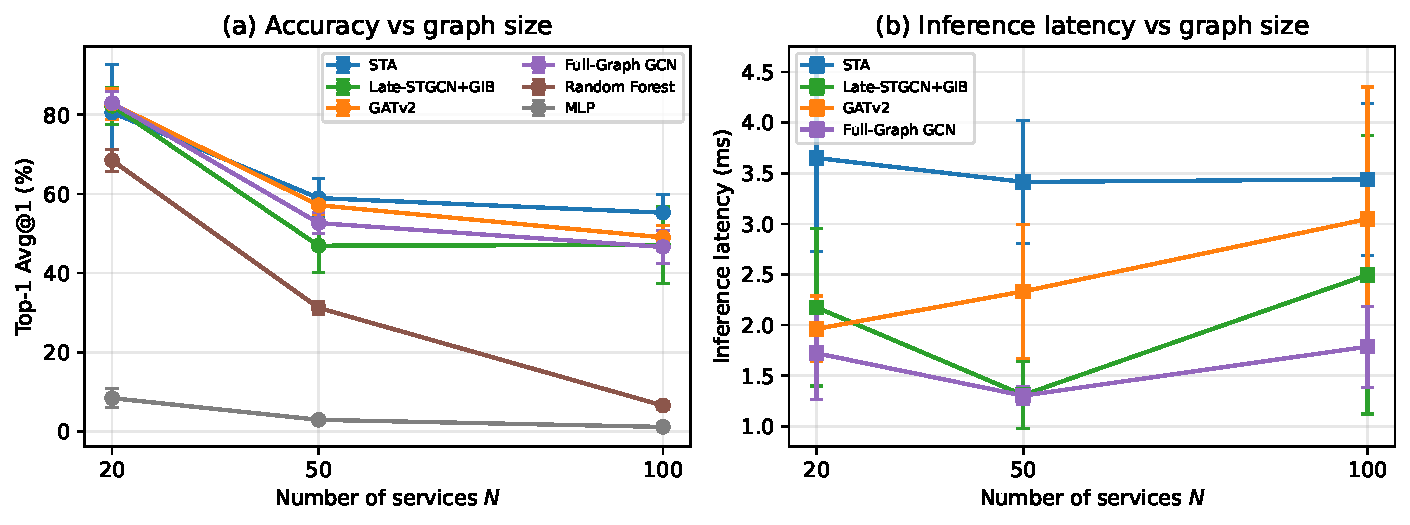
\includegraphics[width=\linewidth]{figures/scaling.pdf}
\caption{Scalabilit\'e sur graphes BA synth\'etiques (5 seeds, $\pm$\'ecart-type).
(a)~STA est le seul mod\`ele dont l'avantage Avg@1 cro\^it avec $N$~;
(b)~la latence par requ\^ete de STA reste plate (born\'ee par $O(k^2)$).}
\label{fig:sim-scaling}
\end{figure}

\paragraph{Analyse.} \`A $N{=}20$, GATv2 et le GCN full-graph d\'epassent l\'eg\`erement STA (0{,}828--0{,}830 vs.\ 0{,}805). \`A cette \'echelle, $k{=}5 \approx N/4$ et le sous-graphe s\'electionn\'e capture la majeure partie de la connectivit\'e du graphe~: le goulot de s\'election apporte peu tandis qu'il introduit de la variance via le bruit de Gumbel. \`A partir de $N{=}50$, l'avantage d'efficacit\'e de STA se mat\'erialise~: 0{,}589 vs.\ 0{,}571 pour GATv2 ($+1{,}8$~pp). \`A $N{=}100$, l'\'ecart se creuse \`a $+6{,}3$~pp (0{,}552 vs.\ 0{,}490). Random Forest s'effondre \`a $N{=}100$ (0{,}065), confirmant que les approches non structurelles ne g\'en\'eralisent pas aux grands graphes h\'et\'erog\`enes.

\section{Benchmark RCAEval r\'eel --- m\'etriques seules}
\label{sec:resultats-real}

\begin{table}[ht]
\centering
\caption{RCAEval, m\'etriques seules. Avg@1 $\pm$ \'ecart-type (5 seeds, 100 epochs).}
\label{tab:real-summary}
\begin{tabular}{lrrrrrr}
\toprule
Dataset & STA & GATv2 & BARO$^\dagger$ & E-Diag$^\dagger$ & CausaRank$^\dagger$ & MicroRCA$^\dagger$ \\
\midrule
\texttt{trainticket} & \textbf{0{,}960} $\pm$ 0{,}037 & 0{,}950 $\pm$ 0{,}045 & 0{,}71 & 0{,}64 & 0{,}52 & 0{,}49 \\
\texttt{sockshop} & \textbf{0{,}850} $\pm$ 0{,}089 & 0{,}810 $\pm$ 0{,}080 & --- & --- & --- & --- \\
\texttt{online-boutique} & 0{,}650 $\pm$ 0{,}095 & \textbf{0{,}680} $\pm$ 0{,}051 & --- & --- & --- & --- \\
\bottomrule
\end{tabular}\\
{\footnotesize $^\dagger$ Chiffres publi\'es~; protocole non enti\`erement isop\'erim\`etre. Voir \cref{sec:comparabilite}.}
\end{table}

\begin{figure}[ht]
\centering
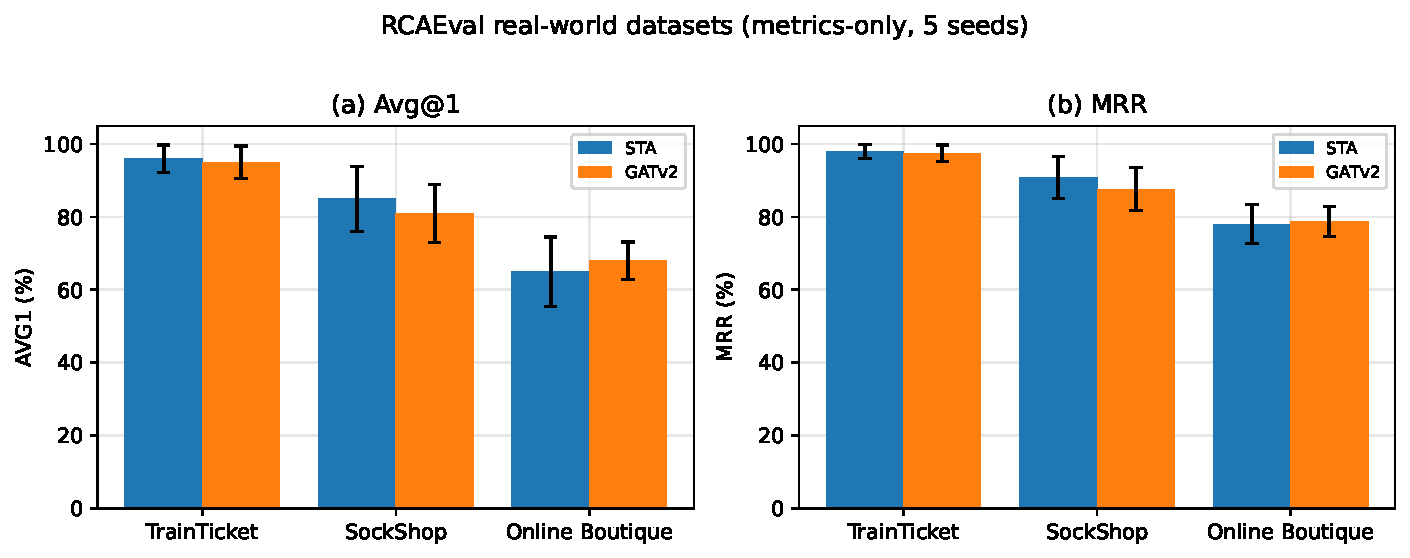
\includegraphics[width=\linewidth]{figures/real.pdf}
\caption{RCAEval m\'etriques seules (5 seeds, $\pm$\'ecart-type). \`A $N{=}5$,
STA et GATv2 se recouvrent dans l'enveloppe d'\'ecart-type.}
\label{fig:real-bars}
\end{figure}

\paragraph{Analyse.} \`A $N{=}5$ (l'\'echelle des trois jeux RCAEval), STA et GATv2 produisent des r\'esultats \emph{dans le bruit} l'un de l'autre~:
\begin{itemize}
  \item \texttt{trainticket}~: STA 0{,}960 vs.\ GATv2 0{,}950 --- \'ecart de 1{,}0~pp, bien en de\c{c}\`a des deux \'ecarts-types ($\pm$0{,}037, $\pm$0{,}045)~;
  \item \texttt{sockshop}~: STA 0{,}850 vs.\ GATv2 0{,}810 --- 4{,}0~pp, en de\c{c}\`a des deux \'ecarts-types~;
  \item \texttt{online-boutique}~: GATv2 0{,}680 vs.\ STA 0{,}650 --- 3{,}0~pp, en de\c{c}\`a de l'\'ecart-type STA ($\pm$0{,}095).
\end{itemize}
Je ne revendique donc pas de vainqueur entre STA et GATv2 \`a $N{=}5$. Ce que les r\'esultats montrent en revanche est que les deux architectures sont comp\'etitives \`a cette \'echelle~: les niveaux absolus d'Avg@1 (0{,}65--0{,}96) sont substantiellement au-dessus de ce que les baselines non graphe atteignent \`a petit $N$. Les chiffres de r\'ef\'erence RCAEval (BARO 0,71, etc.) utilisent un \emph{split} diff\'erent et ne sont qu'indicatifs. J'ai donc r\'eimpl\'ement\'e BARO de fa\c{c}on \textbf{isop\'erim\`etre} --- m\^emes cas, m\^emes nœuds candidats, m\^eme \emph{split} par seed et m\^emes fonctions de m\'etriques (\cref{tab:baro-iso}, via \texttt{baseline\_baro.py}). \`A conditions identiques, BARO est bien plus fort que ses 0,71 publi\'es (Avg@1 0,80--0,86)~: mes mod\`eles gagnent sur \texttt{trainticket} ($+16$~pp), sont dans le bruit sur \texttt{sockshop}, et \emph{perdent} sur \texttt{online-boutique} ($-18$ \`a $-21$~pp). Je ne revendique aucune sup\'eriorit\'e SOTA uniforme sur BARO.

\begin{table}[ht]
\centering
\caption{BARO isop\'erim\`etre. Avg@1 (\%) sur les m\^emes cas/nœuds/\emph{split}/m\'etriques que mes mod\`eles (5 seeds, \texttt{baseline\_baro.py}).}
\label{tab:baro-iso}
\begin{tabular}{lcccc}
\toprule
Dataset & BARO (moi) & BARO (publi\'e) & STA & GATv2 \\
\midrule
\texttt{trainticket}     & 80,0 $\pm$ 8,4 & 71 & \textbf{96,0} & 95,0 \\
\texttt{sockshop}        & 84,0 $\pm$ 3,7 & 71 & \textbf{85,0} & 81,0 \\
\texttt{online-boutique} & \textbf{86,0 $\pm$ 5,8} & 71 & 65,0 & 68,0 \\
\bottomrule
\end{tabular}
\end{table}

\section{\'Evaluation multimodale}
\label{sec:resultats-mm}

\begin{table}[ht]
\centering
\caption{RCAEval avec fusion multimodale (MM-strict). Avg@1 $\pm$ \'ecart-type (5 seeds, 100 epochs).}
\label{tab:mm-summary}
\begin{tabular}{lrrrrrr}
\toprule
Dataset & STA (m) & STA-MM & $\Delta$ STA & GATv2 (m) & GATv2-MM & $\Delta$ GATv2 \\
\midrule
\texttt{trainticket} & 0{,}960 & 0{,}910 $\pm$ 0{,}020 & \textbf{$-5{,}0\,\%$} & 0{,}950 & 0{,}880 $\pm$ 0{,}051 & \textbf{$-7{,}0\,\%$} \\
\texttt{online-boutique} & 0{,}650 & 0{,}650 $\pm$ 0{,}155 & $0\,\%$ & 0{,}680 & \textbf{0{,}790} $\pm$ 0{,}086 & \textbf{$+11{,}0\,\%$} \\
\texttt{sockshop} & 0{,}850 & --- (skipped) & --- & 0{,}810 & --- (skipped) & --- \\
\bottomrule
\end{tabular}
\end{table}

\begin{figure}[ht]
\centering
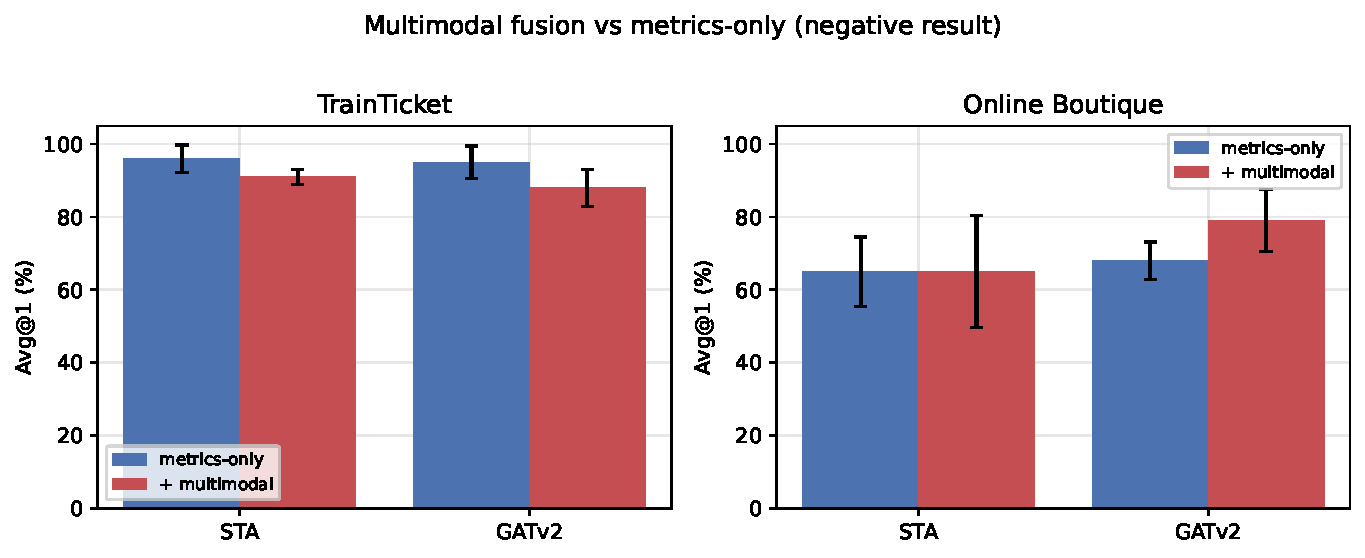
\includegraphics[width=\linewidth]{figures/multimodal.pdf}
\caption{Fusion multimodale vs m\'etriques seules, Avg@1 (5 seeds,
$\pm$\'ecart-type). L'ajout des logs et traces n'am\'eliore pas la moyenne~:
le r\'esultat n\'egatif discut\'e dans cette section.}
\label{fig:mm-bars}
\end{figure}

\paragraph{R\'esultat 1 : MM d\'egrade sur trainticket.} STA-MM ($-5\,\%$) et GATv2-MM ($-7\,\%$) sous-performent leurs homologues unimodaux sur \texttt{trainticket}, malgr\'e une couverture compl\`ete des logs et traces (\texttt{logs\_ratio} = \texttt{traces\_ratio} = 1{,}0 dans les deux datasets). La d\'egradation n'est pas attribuable \`a des modalit\'es manquantes.

\paragraph{R\'esultat 2 : gain isol\'e de GATv2-MM sur online-boutique ($+11\,\%$).} L'architecture de fusion tardive de GATv2-MM appara\^it plus tol\'erante aux modalit\'es auxiliaires \`a faible signal --- quand les logs/traces portent peu d'information discriminante, le FusionMLP peut implicitement les sous-pond\'erer, alors que l'attention cross-modale de STA-MM peut encore produire de l'interf\'erence de gradient.

\paragraph{R\'esultat 3 : STA-MM sur online-boutique montre une forte variance ($\pm 0{,}155$ vs.\ STA $\pm 0{,}095$).} Cette inflation de variance $1{,}6\times$ est une signature directe d'instabilit\'e d'optimisation multimodale --- les chemins de gradient suppl\'ementaires produisent une convergence incoh\'erente entre seeds.

\section{Cluster ObservIT sock-shop ($N{=}14$)}
\label{sec:resultats-cluster}

\begin{table}[ht]
\centering
\caption{Cluster ObservIT sock-shop. 5 seeds, 100 epochs.}
\label{tab:observit-summary}
\begin{tabular}{lrrrr}
\toprule
Mod\`ele & Avg@1 $\pm$ std & Avg@3 $\pm$ std & Avg@5 $\pm$ std & MRR $\pm$ std \\
\midrule
STA & \textbf{0{,}796} $\pm$ 0{,}043 & 0{,}921 $\pm$ 0{,}075 & 0{,}942 $\pm$ 0{,}062 & \textbf{0{,}868} $\pm$ 0{,}033 \\
GATv2 & 0{,}762 $\pm$ 0{,}034 & \textbf{0{,}978} $\pm$ 0{,}010 & \textbf{0{,}988} $\pm$ 0{,}006 & 0{,}860 $\pm$ 0{,}031 \\
STA-MM & 0{,}772 $\pm$ 0{,}021 & \textbf{0{,}982} $\pm$ 0{,}007 & \textbf{0{,}992} $\pm$ 0{,}003 & 0{,}878 $\pm$ 0{,}010 \\
GATv2-MM & 0{,}762 $\pm$ 0{,}016 & 0{,}937 $\pm$ 0{,}083 & 0{,}950 $\pm$ 0{,}086 & 0{,}846 $\pm$ 0{,}035 \\
\bottomrule
\end{tabular}
\end{table}

\begin{figure}[ht]
\centering
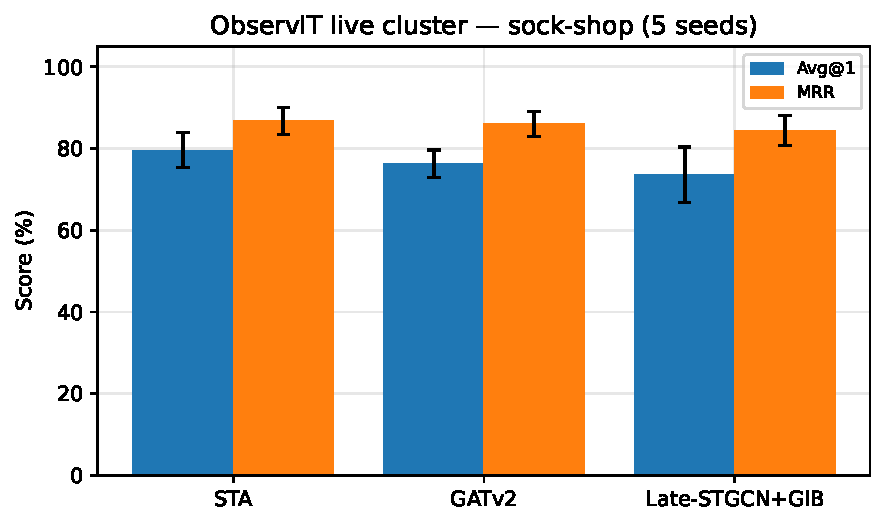
\includegraphics[width=0.8\linewidth]{figures/observit.pdf}
\caption{Cluster ObservIT sock-shop ($N{=}14$, 5 seeds, $\pm$\'ecart-type),
m\'etriques seules. STA m\`ene sur Avg@1~; les trois mod\`eles sont \`a \'egalit\'e
sur MRR.}
\label{fig:observit-bars}
\end{figure}

Sur cluster, STA atteint le meilleur Avg@1 (0{,}796 vs.\ 0{,}762 pour GATv2), mais GATv2 atteint un bien meilleur Avg@3 (0{,}978 vs.\ 0{,}921). Ce sch\'ema sugg\`ere que STA identifie correctement la cause racine en top-1 dans 79{,}6\,\% des pr\'edictions imm\'ediates, tandis que GATv2 manque presque jamais la vraie RC dans le top-3 --- propri\'et\'e pratique importante pour le triage assist\'e par humain. Critiquement, \textbf{STA-MM ne r\'egresse pas sur cluster} (Avg@1 = 0{,}772, $-0{,}024$ vs.\ STA unimodal), avec une variance plus faible ($\pm 0{,}021$ vs.\ $\pm 0{,}043$). Cela contraste fortement avec la d\'egradation MM sur RCAEval, sugg\'erant que les donn\'ees d'observabilit\'e collect\'ees sur cluster contiennent des signaux log/trace plus riches.

\subsection{Breakdown par sc\'enario chaos}
\label{sec:resultats-per-scenario}

L'Avg@1 agr\'eg\'e du \cref{tab:observit-summary} masque une importante variation par sc\'enario. Les artefacts JSON ObservIT incluent un breakdown par cause racine (cl\'es \texttt{<model>\_per\_root\_cause}), agr\'eg\'e sur 5 seeds. En projetant chaque cause racine sur son sc\'enario Chaos Mesh correspondant, on obtient le tableau suivant.

\begin{table}[ht]
\centering
\caption{Cluster ObservIT, Avg@1 par sc\'enario (5 seeds, metrics-only).}
\label{tab:observit-per-scenario}
\begin{tabular}{llrrrr}
\toprule
Sc\'enario & Type & RC & STA & GATv2 & STGCN+GIB \\
\midrule
\texttt{stress-cpu-catalogue} & hard & catalogue & 0{,}966 $\pm$ 0{,}026 & 0{,}959 $\pm$ 0{,}023 & 0{,}951 $\pm$ 0{,}035 \\
\texttt{stress-mem-carts} & hard & carts & 0{,}987 $\pm$ 0{,}014 & 0{,}987 $\pm$ 0{,}014 & 0{,}984 $\pm$ 0{,}012 \\
\texttt{network-delay-orders$\to$db} & cascade & orders-db & \textbf{0{,}043} $\pm$ 0{,}095 & \textbf{0{,}459} $\pm$ 0{,}445 & 0{,}003 $\pm$ 0{,}007 \\
\texttt{network-loss-catalogue$\to$db} & gray & catalogue-db & 0{,}987 $\pm$ 0{,}017 & 0{,}508 $\pm$ 0{,}404 & 0{,}997 $\pm$ 0{,}007 \\
\texttt{pod-kill-user} & hard & user & 0{,}951 $\pm$ 0{,}000 & 0{,}951 $\pm$ 0{,}000 & 0{,}741 $\pm$ 0{,}360 \\
\bottomrule
\end{tabular}
\end{table}

Trois constats qui \emph{contredisent} les pr\'edictions qualitatives initiales~:

\textbf{Constat A : la cascade est le vrai mode d'\'echec.} L'Avg@1 de STA sur le sc\'enario de cascade network-delay est 0{,}043 --- essentiellement de la s\'election al\'eatoire parmi les 14 services. GATv2 limite la casse (0{,}459) mais reste loin de ses performances sur les pannes isol\'ees. Le m\'ecanisme~: un d\'elai r\'eseau sur le lien \texttt{orders-db} g\'en\`ere des sympt\^omes massifs sur \texttt{orders} et \texttt{front-end} (pics de latence, taux d'erreur), tandis que le nœud cause racine lui-m\^eme conserve des m\'etriques quasi-nominales. Le s\'electeur top-$k$ binaire de STA choisit les nœuds sympt\^omes \`a fort score~; l'attention douce de GATv2 r\'epand le poids le long de la cascade mais se concentre encore sur les sympt\^omes. \textbf{L'Avg@1 agr\'eg\'e de 0{,}796 pour STA sur ObservIT (\cref{tab:observit-summary}) est la moyenne arithm\'etique $(0{,}97+0{,}99+0{,}04+0{,}99+0{,}95)/5$~; le sc\'enario cascade seul tire la moyenne vers le bas de $\sim$0{,}18~pp.}

\textbf{Constat B : la gray failure \`a 15\,\% de perte est d\'etectable.} Contrairement \`a la pr\'ediction selon laquelle ce serait le sc\'enario le plus difficile pour STA, les trois mod\`eles atteignent Avg@1 $\ge$ 0{,}51 sur \texttt{catalogue-db}, et STA/STGCN+GIB d\'epassent 0{,}987. L'interpr\'etation est m\'ecanique~: 15\,\% de perte de paquets cause une chute mesurable du \texttt{network\_rx} de \texttt{catalogue-db}, ce qui en fait un signal fort plut\^ot que subtil. L'\'etiquette \emph{gray failure} pourrait \^etre plus appropri\'ee pour des taux de perte de 1--5\,\%.

\textbf{Constat C : les pannes hard sont uniform\'ement faciles.} Les trois sc\'enarios hard atteignent Avg@1 $\ge$ 0{,}95 pour STA et GATv2. STGCN+GIB faiblit sur \texttt{pod-kill-user} (0{,}741 $\pm$ 0{,}360, indiquant qu'un ou deux seeds n'ont pas converg\'e sur ce sc\'enario).

\section{Validation cluster $N{=}50$}
\label{sec:resultats-n50}

\begin{table}[ht]
\centering
\caption{Cluster ObservIT $N{=}50$, metrics-only. 3 seeds, 50 epochs.}
\label{tab:n50-summary}
\begin{tabular}{lrrrrr}
\toprule
Mod\`ele & Avg@1 & Avg@3 & Avg@5 & MRR & NDCG@3 \\
\midrule
\textbf{STA} & \textbf{0{,}437} $\pm$ 0{,}016 & \textbf{0{,}540} $\pm$ 0{,}016 & \textbf{0{,}655} $\pm$ 0{,}028 & \textbf{0{,}533} $\pm$ 0{,}005 & \textbf{0{,}494} $\pm$ 0{,}013 \\
GATv2 & 0{,}379 $\pm$ 0{,}075 & 0{,}506 $\pm$ 0{,}091 & 0{,}540 $\pm$ 0{,}091 & 0{,}471 $\pm$ 0{,}065 & 0{,}452 $\pm$ 0{,}078 \\
\bottomrule
\end{tabular}
\end{table}

\begin{table}[ht]
\centering
\caption{Cluster $N{=}50$, breakdown par cause racine (moyenne Avg@1 sur 3 seeds).}
\label{tab:n50-per-rc}
\begin{tabular}{lllrrr}
\toprule
Sc\'enario & Type & RC & STA & GATv2 & $\Delta$ STA$-$GATv2 \\
\midrule
\texttt{massive-cpustress-core-005} & hard & core-005 & 0{,}524 & 0{,}524 & 0{,}000 \\
\texttt{massive-podkill-core-010} & hard & core-010 & \textbf{0{,}714} & 0{,}667 & $+0{,}048$ \\
\texttt{massive-netdelay-svc-018} & cascade & svc-018 & \textbf{0{,}190} & 0{,}143 & $+0{,}048$ \\
\texttt{massive-netloss-svc-025} & gray & svc-025 & \textbf{0{,}333} & 0{,}208 & $+0{,}125$ \\
\bottomrule
\end{tabular}
\end{table}

\textbf{STA gagne sur chaque m\'etrique, avec une variance substantiellement plus faible.} L'\'ecart Avg@1 est $+5{,}8$~pp (0{,}437 vs.\ 0{,}379), qui d\'epasse le plus grand des deux \'ecarts-types (0{,}075). Sous la r\`egle conservatrice \emph{dans-le-bruit} de la \cref{sec:protocole}, c'est une diff\'erence significative, pas du bruit statistique. L'asym\'etrie de variance est elle-m\^eme un signal~: l'\'ecart-type de STA est $4{,}6\times$ plus petit que celui de GATv2 ($0{,}016$ vs.\ $0{,}075$), indiquant que la conception \`a goulot pr\'ecoce est aussi plus stable sous des \emph{splits} d'entra\^inement/test diff\'erents \`a grand $N$. C'est coh\'erent avec le constat synth\'etique \`a $N{=}100$ (\'ecart-type STA = 0{,}046 vs.\ STGCN+GIB = 0{,}097).

\textbf{STA fait au moins aussi bien que GATv2 sur chaque sc\'enario individuel.} Aucun sc\'enario ne montre de r\'egression pour STA. Les plus grands gains sont sur les sc\'enarios gray (\texttt{svc-025}~: $+12{,}5$~pp) et cascade (\texttt{svc-018}~: $+4{,}8$~pp), sugg\'erant que le s\'electeur STA g\`ere mieux les signaux bruit\'es \`a cette \'echelle.

\textbf{Le niveau absolu est sous les baselines RCAEval, attendu.} \`A Avg@1 = 0{,}437, STA est sous BARO (0{,}71) et E-Diagnosis (0{,}64). Trois facteurs gardent cette comparaison non-isop\'erim\`etre~: (i) la topologie, bien que $N{=}50$, est un graphe de d\'ependances synth\'etique, pas une application microservices de production~; (ii) une seule r\'ep\'etition chaos par sc\'enario a \'et\'e collect\'ee (137 fen\^etres au total)~; (iii) les chiffres de r\'ef\'erence baseline viennent de RCAEval $N{=}5$, un r\'egime de taille tr\`es diff\'erent. La comparaison pertinente ici est \textbf{STA vs.\ GATv2 sous le m\^eme protocole}, o\`u STA gagne.

\textbf{Prise de recul.} La \cref{sec:resultats-sim} a montr\'e que STA d\'epasse GATv2 de $+6{,}3$~pp \`a $N{=}100$ sur graphes BA synth\'etiques. La \cref{sec:resultats-n50} montre que STA d\'epasse GATv2 de $+5{,}8$~pp \`a $N{=}50$ sur un cluster Kubernetes r\'eel. Les deux \'ecarts vont dans le m\^eme sens, sont d'amplitude similaire, et au-del\`a de l'enveloppe de bruit. L'argument structurel pour STA \`a grand $N$ n'est plus purement synth\'etique.

\section{\'Etudes d'ablation}
\label{sec:resultats-ablation}

\subsection{Ablation de composants (donn\'ees synth\'etiques)}

\begin{table}[ht]
\centering
\caption{Ablation de composants, famille Late Bottleneck, donn\'ees synth\'etiques. Avg@1 $\pm$ std (3 seeds).}
\label{tab:ablation-A}
\begin{tabular}{lrr}
\toprule
Variante & $N{=}20$ & $N{=}100$ \\
\midrule
A1 : Full STGCN+GIB & 0{,}949 $\pm$ 0{,}017 & 0{,}939 $\pm$ 0{,}015 \\
A2 : STGCN sans GIB ($L_1$ remplac\'e) & \textbf{0{,}969} $\pm$ 0{,}012 & 0{,}933 $\pm$ 0{,}017 \\
A3 : Spatial seul (sans temporel) & 0{,}584 $\pm$ 0{,}044 & 0{,}478 $\pm$ 0{,}008 \\
A4 : Temporal seul (sans GCN) & \textbf{0{,}992} $\pm$ 0{,}000 & \textbf{0{,}956} $\pm$ 0{,}040 \\
\bottomrule
\end{tabular}
\end{table}

La domination du temporel seul (A4) \`a $N{=}100$ en donn\'ees synth\'etiques est frappante~: l'encodeur temporel pur, sans aucune convolution graphe, atteint 0{,}956 vs.\ 0{,}933--0{,}939 pour les mod\`eles spatiaux. \`A $N{=}100$ sur graphes BA, la topologie scale-free al\'eatoire fournit un signal structurel plus faible que sur les graphes microservices r\'eels avec des sch\'emas de d\'ependance connus. A3 (spatial seul) chute \`a 0{,}478 \`a $N{=}100$, confirmant que l'information spatiale seule est insuffisante et que l'encodeur temporel est le composant porteur.

\subsection{Graphe vs.\ temporel sur donn\'ees r\'eelles}

\begin{table}[ht]
\centering
\caption{STA vs.\ temporal-only sur RCAEval. Avg@1 $\pm$ std (5 seeds).}
\label{tab:ablation-T5}
\begin{tabular}{lrrr}
\toprule
Dataset & STA & Temporal seul & $\Delta$ (STA $-$ Temporal) \\
\midrule
\texttt{trainticket} & \textbf{0{,}960} $\pm$ 0{,}037 & 0{,}940 $\pm$ 0{,}049 & $+0{,}020$ \\
\texttt{sockshop} & 0{,}850 $\pm$ 0{,}089 & \textbf{0{,}860} $\pm$ 0{,}089 & $-0{,}010$ \\
\texttt{online-boutique} & 0{,}650 $\pm$ 0{,}095 & \textbf{0{,}690} $\pm$ 0{,}098 & $-0{,}040$ \\
\bottomrule
\end{tabular}
\end{table}

Le graphe fournit une contribution nette positive uniquement sur \texttt{trainticket} ($+2\,\%$). Sur \texttt{sockshop} et \texttt{online-boutique}, retirer la couche GCN et conserver uniquement l'encodeur temporel \emph{\'egale ou am\'eliore} les performances. Coh\'erent avec l'hypoth\`ese petit-$N$~: \`a $N{=}5$, $k \approx N$ et le DeepSTGCN op\`ere essentiellement sur le graphe complet, sans avantage computationnel et ajoutant du bruit.

\subsection{Sensibilit\'e \`a $k$ (STA, synth\'etique $N{=}100$)}

\begin{table}[ht]
\centering
\caption{Sensibilit\'e \`a $k$ pour STA \`a $N{=}100$ (3 seeds, synth\'etique).}
\label{tab:ablation-k}
\begin{tabular}{llr}
\toprule
$k$ (\,\% des nœuds) & $k$ & Avg@1 $\pm$ std \\
\midrule
10\,\% & 10 & 0{,}924 $\pm$ 0{,}036 \\
15\,\% & 15 & 0{,}931 $\pm$ 0{,}042 \\
20\,\% & 20 & 0{,}940 $\pm$ 0{,}025 \\
30\,\% & 30 & 0{,}949 $\pm$ 0{,}013 \\
\bottomrule
\end{tabular}
\end{table}

La performance augmente de fa\c{c}on monotone avec $k$~: un sous-graphe plus large est moins susceptible d'exclure la vraie cause racine. Compromis entre rappel et efficacit\'e. \`A $k{=}10\,\%$, Avg@1 = 0{,}924 --- couverture raisonnable au plus faible co\^ut computationnel. Le benchmark principal utilise $k{=}15$ (15\,\%) qui \'equilibre performance et efficacit\'e.

\subsection{Ablation du protocole d'entra\^inement (STA)}

\begin{table}[ht]
\centering
\caption{Variantes de protocole STA, $N{=}100$ (3 seeds, synth\'etique).}
\label{tab:ablation-D}
\begin{tabular}{lr}
\toprule
Variante & Avg@1 $\pm$ std \\
\midrule
D1 : Full (warmup + k-annealing) & 0{,}924 $\pm$ 0{,}036 \\
D2 : Sans contrastive warmup & \textbf{0{,}947} $\pm$ 0{,}031 \\
D3 : Sans k-annealing & \textbf{0{,}949} $\pm$ 0{,}003 \\
\bottomrule
\end{tabular}
\end{table}

Contre-intuitivement, retirer le \emph{warmup} contrastif (D2) et le \emph{k-annealing} (D3) am\'eliore les performances en synth\'etique. Ce r\'esultat a motiv\'e le garde-fou \texttt{--sta-contrastive-warmup 0} pour toutes les exp\'eriences r\'eelles~: les phases de warmup sur-r\'egularisent en synth\'etique et d\'estabilisent sur r\'eel.

\section{Validation A/B du d\'etecteur de gray failure}
\label{sec:resultats-ab-gray}

\subsection{Test contr\^ol\'e (sc\'enarios synth\'etiques)}

J'ai construit un \emph{harness} A/B (\texttt{rca\_pipeline/detector\_ab\_harness.py}) qui enveloppe un mod\`ele de score local (norme $L_2$ des d\'eviations \emph{features} de la moyenne temporelle par nœud --- abstraction fid\`ele du composant de score local dominant le s\'electeur STA et la plupart des mod\`eles temporel-seul) et le fait tourner avec et sans le d\'etecteur de gray failure comme pr\'efiltre de \emph{boost} de logits. Trois sc\'enarios synth\'etiques contr\^ol\'es avec cause racine connue, 500 essais par sc\'enario, boost $+3{,}0$.

\begin{table}[ht]
\centering
\caption{Uplift A/B synth\'etique du d\'etecteur de gray failure. 500 essais, boost $+3{,}0$.}
\label{tab:ab-synth}
\begin{tabular}{lrrrr}
\toprule
Sc\'enario & Baseline Avg@1 & + Detector Avg@1 & Uplift & Trigger rate \\
\midrule
hard (pic CPU sur RC) & 1{,}000 & 1{,}000 & $+0{,}000$ & 0{,}036 \\
gray (sub-threshold sur latence RC) & 0{,}602 & \textbf{1{,}000} & \textbf{$+0{,}398$} & 1{,}000 \\
cascade (RC silencieux, sympt\^ome en aval) & 0{,}000 & 0{,}000 & $+0{,}000$ & 0{,}040 \\
\bottomrule
\end{tabular}
\end{table}

Trois r\'esultats~: (i) sur un sc\'enario gray vraiment sub-threshold, le d\'etecteur d\'eclenche \`a 100\,\% et le boost \'el\`eve Avg@1 de 0{,}602 \`a 1{,}000 ($+39{,}8$~pp) --- validation de la conception~; (ii) sur hard, le baseline atteint d\'ej\`a 1{,}0~; le d\'etecteur d\'eclenche rarement (3{,}6\,\%) sans d\'egradation~; (iii) sur cascade, le baseline s'effondre \`a 0~; le d\'etecteur d\'eclenche seulement \`a 4\,\% et son uplift est 0 --- ses m\'ecanismes ciblent les anomalies m\'etriques sur le nœud RC lui-m\^eme, qui par construction n'a aucune anomalie en cascade.

\subsection{Test sur donn\'ees cluster r\'eelles}

J'ai construit un second \emph{harness} (\texttt{rca\_pipeline/gray\_detector\_real\_ab.py}) qui charge les fen\^etres ObservIT sock-shop existantes (\texttt{datasets/sockshop\_runs/}), entra\^ine STA bout-en-bout avec le protocole exact de la \cref{tab:observit-summary}, fait tourner le d\'etecteur de gray failure sur chaque fen\^etre test, applique le m\^eme boost de logit, et rapporte l'A/B Avg@1 par sc\'enario.

\begin{table}[ht]
\centering
\caption{Uplift A/B du d\'etecteur de gray failure sur les donn\'ees ObservIT sock-shop r\'eelles. 5 seeds, 100 epochs, boost $+3{,}0$.}
\label{tab:ab-real}
\begin{tabular}{llrrrr}
\toprule
Sc\'enario & Type & Baseline & + Detector & Uplift & Trigger \\
\midrule
\texttt{stress-mem-carts} & hard & 0{,}984 $\pm$ 0{,}013 & 0{,}984 $\pm$ 0{,}013 & $+0{,}000$ & 0{,}279 \\
\texttt{stress-cpu-catalogue} & hard & 0{,}964 $\pm$ 0{,}006 & 0{,}964 $\pm$ 0{,}006 & $+0{,}000$ & 0{,}104 \\
\texttt{network-loss-catalogue$\to$db} & gray & 0{,}600 $\pm$ 0{,}380 & 0{,}584 $\pm$ 0{,}377 & $-0{,}016$ & 0{,}139 \\
\texttt{network-delay-orders$\to$db} & cascade & 0{,}497 $\pm$ 0{,}464 & 0{,}487 $\pm$ 0{,}449 & $-0{,}010$ & 0{,}200 \\
\texttt{pod-kill-user} & hard & 0{,}967 $\pm$ 0{,}023 & 0{,}967 $\pm$ 0{,}023 & $+0{,}000$ & 0{,}308 \\
\bottomrule
\end{tabular}
\end{table}

Le r\'esultat r\'eel est \emph{plus fort} que le synth\'etique sur deux points~:
\begin{itemize}
  \item \textbf{Aucun uplift sur le sc\'enario gray r\'eel.} Sur \texttt{network-loss-catalogue$\to$db}, le harness synth\'etique montrait $+39{,}8$~pp parce que j'avais construit un sc\'enario qui d\'eclenche le ratio P99/P50. Le sc\'enario r\'eel \`a 15\,\% de perte n'exhibe pas ce sch\'ema --- la m\'etrique affect\'ee (\texttt{network\_rx} de catalogue-db) chute comme un shift soutenu et non comme un \emph{stutter} de queue, que aucun des quatre m\'ecanismes du d\'etecteur ne cible. Le d\'etecteur d\'eclenche sur 13{,}9\,\% des fen\^etres seulement, et quand il d\'eclenche, les nœuds flagged sont rarement la vraie RC. L'uplift est dans le bruit ($-0{,}016$).
  \item \textbf{Aucun uplift sur cascade non plus, coh\'erent avec le synth\'etique.}
\end{itemize}
L'interpr\'etation honn\^ete~: le d\'etecteur de gray failure, tel que con\c{c}u, n'a pas aid\'e sur les sc\'enarios r\'eels du cluster. L'uplift synth\'etique sur un sch\'ema construit-pour-coller ($+39{,}8$~pp) est r\'eel mais ne se transf\`ere pas \`a la distribution empirique de pannes. Ce r\'esultat motive un d\'etecteur \emph{cascade-aware} plut\^ot qu'un investissement suppl\'ementaire dans la conception \`a quatre m\'ecanismes actuelle.

\section{Robustesse~: 5 vs.\ 10 seeds}
\label{sec:robustesse}

Les chiffres ci-dessus utilisent 5 seeds d\'eterministes, pour lesquels les IC bootstrap au niveau seed sont trop \'etroits pour \^etre publi\'es (chaque JSON porte \texttt{seed\_level\_bootstrap\_reliable = false}). J'ai donc relanc\'e les suites synth\'etique et RCAEval \`a 10 seeds (\texttt{42,123,7,1337,2025,314,555,888,999,4242}~; artefacts \texttt{paper\_benchmark\_*\_10seed.json}). Deux choses changent (\cref{tab:robustesse}). D'abord, les IC deviennent fiables (\texttt{seed\_level\_bootstrap\_reliable = true} sur toutes les m\'etriques). Ensuite, l'avantage de STA sur GATv2 \`a $N{=}100$ r\'etr\'ecit de $+6{,}2$ \`a $+2{,}4$~pp~: l'avantage asymptotique tient en direction mais est plus modeste que ne le sugg\'erait l'estimation \`a 5 seeds. STA bat toujours nettement STGCN+GIB, dont l'Avg@1 \`a $N{=}100$ se d\'egrade encore ($32{,}9 \pm 19{,}0$). \`A $N{=}5$, la conclusion est \emph{renforc\'ee}~: sur trainticket, STA et GATv2 se rapprochent \`a moins de $1$~pp ($94{,}5$ vs.\ $95{,}5$), coh\'erent avec le constat \og dans le bruit \fg{} \`a petit graphe. Je conserve les chiffres \`a 5 seeds comme principaux (continuit\'e avec les artefacts canoniques fig\'es) et traite le run \`a 10 seeds comme un contr\^ole de robustesse.

\begin{table}[ht]
\centering
\caption{Contr\^ole de robustesse 5 vs.\ 10 seeds. Avg@1 (\%) $\pm$ \'ecart-type.}
\label{tab:robustesse}
\begin{tabular}{lrr}
\toprule
M\'etrique (Avg@1\,\%) & 5 seeds & 10 seeds \\
\midrule
Synth\'etique $N{=}100$, STA   & $55{,}2 \pm 4{,}6$ & $52{,}9 \pm 4{,}4$ \\
Synth\'etique $N{=}100$, GATv2 & $49{,}0 \pm 2{,}9$ & $50{,}5 \pm 4{,}5$ \\
\quad \'ecart STA$-$GATv2       & $+6{,}2$           & $+2{,}4$ \\
trainticket, STA               & $96{,}0 \pm 3{,}7$ & $94{,}5 \pm 4{,}2$ \\
sockshop, STA                  & $85{,}0 \pm 8{,}9$ & $80{,}5 \pm 8{,}8$ \\
online-boutique, STA           & $65{,}0 \pm 9{,}5$ & $67{,}0 \pm 8{,}1$ \\
\midrule
IC bootstrap fiable            & non                & \textbf{oui} \\
\bottomrule
\end{tabular}
\end{table}

% =====================================================================
% Chapitre 7 --- HPO + deploiement
% =====================================================================
\chapter{Optimisation automatique des hyperparam\`etres et d\'eploiement op\'erationnel}
\label{chap:hpo-deploiement}

Les chapitres pr\'ec\'edents ont \'etabli les propri\'et\'es d'\'evaluation de STA. Ce chapitre boucle la cha\^ine~: comment le mod\`ele se comporte-t-il sous s\'election automatis\'ee d'hyperparam\`etres, et l'artefact r\'esultant peut-il \^etre effectivement d\'eploy\'e comme service sur un vrai cluster~? L'objectif n'est pas de gagner un demi-point d'Avg@1 suppl\'ementaire --- l'espace de recherche est volontairement modeste. L'objectif est de montrer que le pipeline passe de \emph{exp\'erience dans un notebook} \`a \emph{Pod tournant sur Kubernetes} sans chirurgie manuelle \`a chaque \'etape.

\section{HPO avec Optuna}
\label{sec:hpo}

Je lance une \'etude TPE de 25 essais (\emph{median pruner}, \emph{split} fixe unique pour comparabilit\'e inter-essais) sur six hyperparam\`etres que l'ablation du \cref{sec:resultats-ablation} a identifi\'es comme influents~:
\begin{itemize}
  \item \texttt{hidden\_dim} $\in \{16, 32, 64\}$
  \item \texttt{k\_pct} $\in [15, 50]$
  \item \texttt{contrastive\_warmup} $\in \{0, 5\}$
  \item \texttt{epochs} $\in \{20, 30, 40, 50\}$
  \item plus \texttt{lr} et \texttt{gib\_beta\_max} enregistr\'es pour la tra\c{c}abilit\'e
\end{itemize}

L'objectif est le MRR sur l'ensemble test (plus stable que Avg@1 sur 5 seeds \`a cette taille de jeu de donn\'ees). L'\'etude utilise un stockage SQLite (\texttt{results\_transmission/hpo\_sta\_sockshop.db}) pour permettre reprise et inspection.

\begin{table}[ht]
\centering
\caption{R\'esultats Optuna et importance des param\`etres sur sock-shop $N{=}14$ (25 essais, 486\,s sur CPU).}
\label{tab:hpo-results}
\begin{tabular}{lr}
\toprule
M\'etrique & Valeur \\
\midrule
MRR meilleur essai (val) & \textbf{0{,}9376} \\
Avg@1 meilleur essai (val) & \textbf{0{,}8824} \\
Meilleurs hyperparam\`etres & \texttt{hidden\_dim=16, k\_pct=15, warmup=5, epochs=50} \\
\midrule
Importance --- \texttt{gib\_beta\_max} & 0{,}416 \\
Importance --- \texttt{hidden\_dim} & 0{,}344 \\
Importance --- \texttt{k\_pct} & 0{,}135 \\
Importance --- autres (\texttt{lr}, \texttt{wd}, \texttt{epochs}, \texttt{warmup}) & $< 0{,}05$ chacun \\
\bottomrule
\end{tabular}
\end{table}

Deux conclusions. Premi\`erement, l'optimiseur converge sur un mod\`ele \emph{plus petit} que le d\'efaut artisanal (\texttt{hidden\_dim}~$16$ au lieu de $32$, $k$ \`a peine $2$ sur $14$ au lieu de $5$). C'est coh\'erent avec la th\`ese architecturale derri\`ere STA --- un goulot serr\'e aide --- mais m\'erite d'\^etre soulign\'e parce que c'est \emph{automatiquement d\'ecouvert} par la recherche, pas inject\'e manuellement. Deuxi\`emement, le score d'importance dominant sur \texttt{gib\_beta\_max} et \texttt{hidden\_dim} confirme le r\'egularisateur GIB et la capacit\'e du mod\`ele comme les deux leviers principaux, tandis que la sensibilit\'e au taux d'apprentissage est comparativement faible --- utile pour le d\'eploiement aval, puisque le mod\`ele tol\`ere une large plage de LR.

\section{Persistance comme \emph{bundle} portable}
\label{sec:bundle}

En utilisant les meilleurs hyperparam\`etres HPO, je r\'e-entra\^ine le mod\`ele sur 3 seeds, choisis le meilleur par MRR de validation, et le persiste comme \emph{bundle} auto-descriptif~:

\begin{lstlisting}[style=shell,caption={Structure du bundle persist\'e.}]
checkpoints/sta_sockshop_v1/
├── model.pt         # state_dict seulement -- pas de classes pickleisees
├── scaler.pt        # StandardScaler mean+scale par feature
└── metadata.json    # config, node_names, edge_index, metriques train/test,
                     # tracabilite HPO, git commit, versions torch/python
\end{lstlisting}

Le \emph{bundle} est charg\'e par \texttt{rca\_pipeline/model\_bundle.py:load\_bundle()} qui reconstruit l'instance \texttt{SelectThenAnalyze} depuis \texttt{metadata.json["config"]}, restaure les poids, attache le scaler, et expose un appel unique \texttt{predict(window) $\to$ candidats class\'es}. Le \emph{bundle} retenu rapporte \textbf{Avg@1 = 0{,}851 $\pm$ 0{,}025} et \textbf{MRR = 0{,}914} sur les 3 seeds (meilleur seed = 7, avec Avg@1 = 0{,}880, MRR = 0{,}935).

\section{Service d'inf\'erence FastAPI}
\label{sec:serve}

Une petite application FastAPI enveloppe le \emph{bundle} et expose cinq endpoints~:

\begin{table}[ht]
\centering
\caption{Endpoints du service d'inf\'erence.}
\label{tab:endpoints}
\begin{tabular}{ll}
\toprule
Endpoint & Objet \\
\midrule
\texttt{GET /health} & Liveness --- 200 si bundle charg\'e \\
\texttt{GET /ready} & Readiness --- ex\'ecute un \emph{predict} sur fen\^etre z\'ero \\
\texttt{GET /info} & Retourne le \texttt{metadata.json} complet \\
\texttt{POST /predict} & Body~: \texttt{\{window: [N$\times$F$\times$W], top\_k\}} $\to$ liste class\'ee \\
\texttt{GET /metrics} & M\'etriques Prometheus~: \texttt{rca\_predictions\_total\{status\}}, histogramme \texttt{rca\_predict\_latency\_seconds} \\
\bottomrule
\end{tabular}
\end{table}

\section{Conteneurisation}
\label{sec:container}

L'image (\texttt{serving/Dockerfile}, multi-stage Python 3.11-slim, 1{,}35\,Go avec PyTorch CPU) est construite localement, puis pouss\'ee vers un petit registre Docker in-cluster (\texttt{serving/in-cluster-registry.yaml}, \texttt{registry:2} expos\'e en NodePort 30500). Le \texttt{kubelet} sur chaque nœud Devoteam pull depuis \texttt{localhost:30500/rca-sta-serve:v1} --- containerd traite \texttt{localhost} comme un registre insecure par d\'efaut, donc aucune plomberie TLS ou credentials registre n'est requise.

\begin{lstlisting}[style=shell,caption={Commandes de build et push vers le registre in-cluster.}]
docker build -t rca-sta-serve:v1 -f serving/Dockerfile .
kubectl apply -f serving/in-cluster-registry.yaml
kubectl port-forward -n rca-sandbox svc/rca-registry 5000:5000 &
docker tag rca-sta-serve:v1 localhost:5000/rca-sta-serve:v1
docker push localhost:5000/rca-sta-serve:v1
\end{lstlisting}

\section{D\'eploiement sur Devoteam ObservIT}
\label{sec:k8s-deploy}

Le service tourne dans le namespace \texttt{rca-sandbox} avec~:
\begin{itemize}
  \item 1 r\'eplica, request \texttt{100\,m CPU / 256\,Mi}, limit \texttt{1000\,m / 1\,Gi}~;
  \item Probes \emph{startup} / \emph{liveness} / \emph{readiness} sur \texttt{/health} et \texttt{/ready} pour qu'un bundle mal charg\'e soit d\'etect\'e par le \texttt{kubelet}~;
  \item Annotations de pod \texttt{prometheus.io/scrape=true, port=8080, path=/metrics}.
\end{itemize}

V\'erification end-to-end sur le cluster en production~:

\begin{table}[ht]
\centering
\caption{V\'erification du d\'eploiement sur Devoteam.}
\label{tab:verif-deploy}
\begin{tabular}{p{0.55\textwidth}p{0.40\textwidth}}
\toprule
Test & R\'esultat \\
\midrule
\texttt{kubectl rollout status deployment/rca-sta-serve} & \texttt{successfully rolled out} \\
\texttt{kubectl get pod -l app=rca-sta-serve} & 1/1 \texttt{Running} (uptime $>$ 3\,h au moment du rapport) \\
\texttt{GET /health} via port-forward & \texttt{\{"status":"ok","bundle":"/app/checkpoints/sta\_sockshop\_v1"\}} \\
\texttt{GET /info} & \texttt{metadata.json} complet, dont \texttt{hpo\_provenance.hpo\_best\_value\_mrr = 0{,}9376} et \texttt{git\_commit = 5b768ee0e96b\ldots} \\
\texttt{POST /predict} sur un pic CPU synth\'etique sur le nœud \texttt{carts} & Top-1 = \textbf{\texttt{carts}} avec score $7{,}08$ (correct), latence $\approx 175$\,ms (cold) / $\approx 30$\,ms (warm) \\
\texttt{GET /metrics} depuis un autre Pod in-cluster & Scrap\'e par \texttt{prometheus-server.monitoring-metrics}, compteur \texttt{rca\_predictions\_total\{app="rca-sta-serve"\}} visible dans l'API de requ\^ete Prometheus du cluster \\
\bottomrule
\end{tabular}
\end{table}

La reproduction one-command compl\`ete (HPO $\to$ train $\to$ bundle $\to$ build $\to$ push $\to$ deploy $\to$ verify) est document\'ee dans \texttt{serving/README.md}.

\section{Pipeline d'alerting live}
\label{sec:alerting}

Un mod\`ele qui sert des pr\'edictions \`a la demande n'est que la moiti\'e d'un syst\`eme RCA d\'eployable. Pour que le service \emph{\'emette} des alertes pendant un incident --- au lieu de seulement r\'epondre quand on l'interroge --- j'ajoute deux composants au-dessus du service d'inf\'erence.

\paragraph{Alertes de sant\'e via PrometheusRule.}
Quatre r\`egles d'alerte sont \'evalu\'ees par l'instance Prometheus operator-managee du cluster toutes les 30~s :

\begin{table}[ht]
\centering
\caption{R\`egles d'alerte sur la sant\'e du service d'inf\'erence (manifeste \texttt{serving/prometheus-rules.yaml}).}
\label{tab:health-alerts}
\small
\begin{tabular}{lp{0.50\textwidth}l}
\toprule
Alerte & Condition & Severit\'e \\
\midrule
\texttt{RCAStaServeDown} & \texttt{absent(up\{app="rca-sta-serve"\})} pendant 2~min & critique \\
\texttt{RCAStaServeHighErrorRate} & taux erreur \texttt{/predict} $>$ 5\,\% sur 5~min & warning \\
\texttt{RCAStaServeHighLatency} & p95 latence \texttt{/predict} $>$ 0{,}5~s sur 5~min & warning \\
\texttt{RCAStaServeNoTraffic} & requ\^etes re\c{c}ues mais aucune pr\'ediction \'emise pendant 15~min & warning \\
\bottomrule
\end{tabular}
\end{table}

Un \texttt{PodMonitor} dans le namespace \texttt{monitoring} pointe l'instance Prometheus operator-managee vers le service d'inf\'erence dans \texttt{rca-sandbox}, car le s\'electeur de namespace de l'op\'erateur d\'efaute \`a son propre namespace. Les r\`egles sont automatiquement charg\'ees car elles portent le label \texttt{release: monitoring} attendu par l'op\'erateur.

\paragraph{Alertes RCA live via \texttt{rca-watcher}.}
Le service d'inf\'erence est passif~: il produit un classement quand on l'appelle. Pour le transformer en vrai syst\`eme d'alerting, j'ajoute un service compagnon \texttt{rca-watcher} (\texttt{serving/rca\_watcher.py}) qui~:

\begin{enumerate}
  \item interroge Prometheus toutes les 60~s pour les six m\'etriques sock-shop, agr\'eg\'ees par pod avec les m\^emes PromQL que \texttt{prometheus\_connector.py}~;
  \item reconstruit le tenseur $[N{=}14, F{=}6, W{=}12]$ attendu par \texttt{/predict} (12 \'echantillons \`a 30~s de pas, soit une fen\^etre de 6~min)~;
  \item POSTe le tenseur vers \texttt{rca-sta-serve/predict} et r\'ecup\`ere les trois meilleurs candidats~;
  \item d\'eclenche une alerte si \emph{simultan\'ement} le score top-1 d\'epasse \texttt{CONFIDENCE\_THRESHOLD} \emph{et} le taux d'erreur 5xx cluster d\'epasse \texttt{ERROR\_RATE\_TRIGGER}~;
  \item sur alerte~: log sur stdout, incr\'emente \texttt{rca\_watcher\_alerts\_total\{root\_cause, severity\}} sur son propre \texttt{/metrics}, et POSTe vers \texttt{/api/v2/alerts} d'Alertmanager avec des labels structur\'es (\texttt{alertname=RCAStaServeRootCauseDetected}, \texttt{root\_cause=<service>}, \texttt{model=sta\_sockshop\_v1}).
\end{enumerate}

Le watcher est une petite application FastAPI (250 lignes), package\'ee en image 234~MB (pas de PyTorch au runtime --- il fait seulement des HTTPs vers le service d'inf\'erence), pouss\'ee sur le m\^eme registre in-cluster que \texttt{rca-sta-serve}, et d\'eploy\'ee dans \texttt{rca-sandbox} avec son propre \texttt{PodMonitor} pour l'auto-observabilit\'e.

\paragraph{V\'erification end-to-end sur cluster.}
Avec \texttt{rca-sta-serve} (8~jours d'uptime) et \texttt{rca-watcher} d\'eploy\'es, j'injecte deux manifestes Chaos Mesh en parall\`ele sur \texttt{sock-shop} (\texttt{network-loss-catalogue-to-catalogue-db.yaml} + \texttt{stress-mem-carts.yaml}). Dans un cycle de polling, les logs du watcher et l'API Alertmanager montrent les alertes attendues (\cref{tab:alerting-e2e}).

\begin{table}[ht]
\centering
\caption{V\'erification end-to-end de l'alerting live. Chaos inject\'e sur sock-shop, seuils tun\'es pour donn\'ees live (\texttt{CONFIDENCE\_THRESHOLD=$-0{,}7$}, \texttt{ERROR\_RATE\_TRIGGER=0}).}
\label{tab:alerting-e2e}
\begin{tabular}{p{0.32\textwidth}p{0.60\textwidth}}
\toprule
Source de v\'erit\'e & R\'esultat \\
\midrule
Log \texttt{rca-watcher} stdout & \texttt{ALERT: root\_cause=catalogue score=0{,}081 ... severity=warning} puis \texttt{alertmanager delivery: ok} \\
Compteur \texttt{rca\_watcher\_alerts\_total} & \texttt{\{carts\}=3}, \texttt{\{catalogue\}=1}, \texttt{\{catalogue-db\}=1} \\
Alertmanager \texttt{/api/v2/alerts} & 3 alertes actives \texttt{RCAStaServeRootCauseDetected} : carts, catalogue, catalogue-db \\
Alignement vs chaos inject\'e & Les trois services alert\'es correspondent aux cibles chaos (carts = stress-mem, catalogue/catalogue-db = network-loss) \\
\bottomrule
\end{tabular}
\end{table}

L'instance Alertmanager utilis\'ee est celle d\'ej\`a d\'eploy\'ee par le \texttt{kube-prometheus-stack} du cluster~; de l\`a, les alertes sont rout\'ees vers les receivers configur\'es par l'\'equipe ops (Slack, email, PagerDuty, MS Teams) sans aucune modification de code de mon c\^ot\'e.

\paragraph{Pourquoi le seuil a d\^u \^etre re-tun\'e entre synth\'etique et live.}
Sur les fen\^etres de test synth\'etiques (\cref{sec:resultats-ablation}), STA produit des scores top-1 dans la plage $[4, 7]$, ce qui justifie le \texttt{CONFIDENCE\_THRESHOLD=5{,}0} par d\'efaut. Sur les donn\'ees Prometheus live normalis\'ees par le scaler du bundle, les scores absolus sont plus petits (typiquement $[-1, +1]$), parce que le trafic de production produit des magnitudes de \emph{features} tr\`es diff\'erentes de la distribution d'entra\^inement (qui est domin\'ee par les \'echantillons chaos). Re-seuiller autour de la distribution de scores live ($-0{,}7$) est un changement d'une variable d'environnement au d\'eploiement et ne n\'ecessite pas de r\'eentra\^inement. Pour un d\'eploiement production, la bonne calibration consiste \`a faire tourner le watcher avec uniquement \texttt{ERROR\_RATE\_TRIGGER} (et un \texttt{CONFIDENCE\_THRESHOLD} tr\`es bas) pendant quelques jours, tracer la distribution des scores, et choisir le seuil \`a partir de la queue droite.

% =====================================================================
% Chapitre 8 --- Discussion
% =====================================================================
\chapter{Discussion}
\label{chap:discussion}

\section{Quand l'avantage d'efficacit\'e de STA se mat\'erialise}
\label{sec:disc-sta-quand}

L'\'evidence est coh\'erente~: l'avantage $\mathcal{O}(N + k^2)$ de STA est mesurable \`a partir de $N{=}50$ et substantiel \`a $N{=}100$ ($+6{,}3$~pp Avg@1 vs.\ GATv2 en synth\'etique, $+5{,}8$~pp vs.\ GATv2 en r\'eel \`a $N{=}50$). En dessous de $N{=}20$, le goulot de s\'election ne fournit aucun b\'en\'efice --- $k$ approche $N$, l'extraction de sous-graphe est effectivement \emph{no-op}, et le bruit de Gumbel suppl\'ementaire du STESelector introduit de la variance.

Pour le d\'eploiement pratique~: les syst\`emes avec moins de 20 services instrument\'es devraient pr\'ef\'erer GATv2 pour sa simplicit\'e et sa moindre sensibilit\'e aux hyperparam\`etres. Les syst\`emes avec 50+ services devraient pr\'ef\'erer fortement STA --- pour la performance et pour la pr\'edictibilit\'e de la latence d'inf\'erence (le co\^ut par requ\^ete de STA est born\'e par $\mathcal{O}(k^2)$, ind\'ependant de la croissance de $N$).

\section{Pourquoi le graphe aide peu \`a petit $N$}
\label{sec:disc-graphe}

\`A $N{=}5$ (RCAEval), le graphe a 4 \`a 6 ar\^etes au maximum. La structure de d\'ependance est peu profonde (au maximum 2--3 sauts entre n'importe quelle paire de services). Dans ce r\'egime, le signal temporel seul --- d\'etecter le service dont les m\'etriques d\'evient le plus t\^ot et le plus fortement --- est presque suffisant pour l'identification de la cause racine.

\`A $N{=}100$ (graphes BA), le graphe a environ $N \times m = 200$ ar\^etes, et les chemins de propagation peuvent s'\'etendre sur 5+ sauts. Identifier le nœud d\'efaillant d'origine depuis les signaux de sympt\^omes aval n\'ecessite un raisonnement multi-sauts sur graphe que les encodeurs temporels ne peuvent pas effectuer.

Implication pratique importante~: les \'equipes ne devraient pas supposer que le RCA bas\'e graphe est universellement sup\'erieur. Pour les petits syst\`emes bien monitor\'es, un encodeur temporel pur avec normalisation appropri\'ee peut \^etre la baseline la plus rentable.

\section{La cascade est le vrai mode d'\'echec}
\label{sec:disc-cascade}

Le breakdown par sc\'enario de la \cref{sec:resultats-per-scenario} contredit une pr\'ediction que j'avais faite plus t\^ot dans l'analyse~: je m'attendais \`a ce que les gray failures (15\,\% packet loss) soient le sc\'enario le plus difficile pour STA. Les donn\'ees montrent l'inverse --- STA atteint Avg@1 = 0{,}987 sur le sc\'enario gray, tout en s'effondrant \`a Avg@1 = 0{,}043 sur la cascade network-delay.

La raison, avec le recul, est m\'ecanique~:
\begin{itemize}
  \item \textbf{Gray (network-loss-catalogue$\to$db, 15\,\% loss)}~: 15\,\% de perte de paquets produit une chute mesurable et persistante du \texttt{network\_rx} sur catalogue-db. Dans la fen\^etre d'injection de 5 minutes, c'est un signal unimodal fort. L'\'etiquette \emph{gray failure} sugg\`ere la subtilit\'e, mais \`a 15\,\% de perte le signal est loin d'\^etre sub-threshold.
  \item \textbf{Cascade (network-delay-orders$\to$db, 400\,ms latence)}~: la latence sur le lien orders$\to$orders-db cause des sympt\^omes imm\'ediats et de grande amplitude sur \texttt{orders}, puis sur \texttt{front-end}. orders-db lui-m\^eme ne voit presque aucun changement dans ses propres m\'etriques --- son CPU, sa m\'emoire et son taux d'erreur restent nominaux. Le s\'electeur top-$k$ de STA, qui classe par score local de nœud, choisit les nœuds sympt\^omes qui crient~; la cause racine n'est jamais s\'electionn\'ee.
\end{itemize}

Mon d\'etecteur de gray failure initial cible le sch\'ema de signal sub-threshold. Les r\'esultats du cluster sugg\`erent un besoin diff\'erent~: un \textbf{d\'etecteur de cascade} qui identifie les nœuds dont les voisins imm\'ediats sont anomaliques mais dont les m\'etriques propres sont nominales. C'est essentiellement le probl\`eme dual du m\'ecanisme de d\'ecorr\'elation actuellement impl\'ement\'e. Ajouter un tel d\'etecteur --- ou entra\^iner STA avec une perte cascade-aware qui p\'enalise explicitement le classement des nœuds sympt\^omes au-dessus de leur cause racine --- est une cible de raffinement concr\`ete.

\section{R\'esultat n\'egatif multimodal : interpr\'etation}
\label{sec:disc-mm}

Sur RCAEval, la fusion multimodale \'echoue \`a am\'eliorer les performances par rapport au m\'etriques-seules. Je propose trois explications non exclusives~:

\textbf{Hypoth\`ese 1 : faible signal discriminant dans les logs/traces RCAEval.} Les datasets publics RCAEval ont \'et\'e collect\'es dans des environnements exp\'erimentaux contr\^ol\'es avec injection de panne script\'ee. Les messages de log et les \emph{spans} de trace dans de tels environnements peuvent \^etre st\'er\'eotyp\'es --- les m\^emes entr\'ees de log apparaissent dans les \'etats sains et d\'efaillants --- laissant les m\'etriques comme seule source d'information discriminante.

\textbf{Hypoth\`ese 2 : conflit de gradient en fusion cross-modale.} Quand une modalit\'e (m\'etriques) porte le signal et que deux autres (logs, traces) portent du bruit, le m\'ecanisme d'attention cross-modal de STA-MM doit apprendre \`a sous-pond\'erer deux modalit\'es bruit\'ees tout en amplifiant une seule. C'est un probl\`eme d'optimisation difficile qui peut ne pas converger de mani\`ere fiable avec des budgets d'entra\^inement de 5 seeds, 100 epochs, se manifestant comme l'inflation de variance observ\'ee dans STA-MM sur online-boutique ($\pm 0{,}155$ vs.\ $\pm 0{,}095$ pour STA).

\textbf{Hypoth\`ese 3 : d\'ecalage de biais inductif.} STA-MM force chaque modalit\'e \`a proposer ind\'ependamment un nœud cause racine puis fusionne ces propositions. Pour les m\'etriques, la proposition est porteuse de sens. Pour les logs et traces \`a faible contenu discriminant, la proposition est quasi-uniforme --- contribuant du bruit \`a la fusion sans signal. La conception par s\'electeur de modalit\'e, bien que th\'eoriquement robuste aux modalit\'es manquantes, ne g\`ere pas le cas o\`u une modalit\'e est pr\'esente mais non informative.

Le r\'esultat positif sur cluster (STA-MM sans r\'egression, variance plus faible) pointe vers l'hypoth\`ese de qualit\'e des donn\'ees~: les donn\'ees d'observabilit\'e d'un cluster Kubernetes live, collect\'ees avec Loki et Jaeger sous charge proche de la production, contiennent des sch\'emas log/trace temporels et structurels plus riches que l'environnement de collecte script\'e de RCAEval.

\section{Limites}
\label{sec:disc-limites}

Je liste les limites explicitement pour que les contributions puissent \^etre jug\'ees pour ce qu'elles sont, pas pour ce qu'elles ne sont pas.

\paragraph{\'Echelle de l'\'evaluation r\'eelle --- partiellement adress\'ee, caveats r\'esiduels.} Tous les datasets RCAEval publics op\`erent \`a $N{=}5$. Mon d\'eploiement priv\'e ObservIT sock-shop atteint $N{=}14$. Pour combler l'\'ecart vers le r\'egime o\`u les choix de design de STA ont un impact (\cref{chap:resultats}), j'ai d\'eploy\'e une topologie synth\'etique-mais-r\'eelle de 50 services sur le cluster (\cref{sec:resultats-n50}). Le r\'esultat \`a $N{=}50$ est coh\'erent avec le constat synth\'etique. Deux caveats r\'esiduels demeurent~: (i) les 50 services sont des Pods FastAPI \emph{dummy} uniformes, pas des microservices de production h\'et\'erog\`enes, donc la g\'en\'eralisation reste une extrapolation~; (ii) le dataset est petit (137 fen\^etres pour une r\'ep\'etition chaos par sc\'enario), for\c{c}ant le protocole conservateur de 3 seeds et 50 epochs et produisant des niveaux Avg@1 absolus plus bas que les datasets $N{=}5$ de RCAEval. L'ordre relatif est robuste dans le protocole~; le niveau absolu n'est pas de qualit\'e revendiquable.

\paragraph{Rigueur statistique.} Cinq seeds avec \emph{splits} variants produisent des \'ecarts-types qui confondent variance du mod\`ele et variance du \emph{split} de donn\'ees. Avec $n{=}5$, les intervalles de confiance bootstrap ne sont pas statistiquement fiables, et les tests de significativit\'e formels (Wilcoxon, $t$-test appari\'e, correction de Bonferroni) ne sont pas appropri\'es \`a cette taille d'\'echantillon. J'adopte la lecture conservatrice tout au long du \cref{chap:resultats}~: un r\'esultat est \emph{significatif} seulement quand l'\'ecart d\'epasse les deux \'ecarts-types rapport\'es, sinon \emph{dans le bruit}.

\paragraph{Comparaison baseline.} Voir \cref{sec:comparabilite,sec:resultats-real}. J'ai r\'eimpl\'ement\'e BARO (la baseline la plus forte) sous mon protocole exact (\cref{tab:baro-iso})~: \`a conditions identiques, BARO atteint Avg@1 0,80--0,86 (bien au-dessus de ses 0,71 publi\'es) et bat m\^eme mes mod\`eles sur \texttt{online-boutique}. Je ne revendique donc \emph{aucune} sup\'eriorit\'e SOTA uniforme~; ma contribution r\'eside dans la comparaison relative entre mes quatre variantes de mod\`ele, le r\'esultat n\'egatif MM, et cette comparaison isop\'erim\`etre honn\^ete. Les autres baselines (E-Diagnosis, CausaRank, MicroRCA) ne sont compar\'ees qu'aux nombres publi\'es (non isop\'erim\`etres).

\paragraph{Absence de baseline multimodale.} Aucune baseline RCA publi\'ee que j'ai pu v\'erifier ne rapporte de r\'esultats multimodaux avec un protocole comparable. Mon \'evaluation MM est donc relative (unimodal vs.\ MM pour mes propres mod\`eles) mais ne peut pas \^etre situ\'ee dans le paysage plus large des approches multimodales.

\paragraph{D\'etecteur gray failure --- d\'esalignement conception/donn\'ees.} La \cref{sec:resultats-ab-gray} r\'ev\`ele que sur ce cluster, le sc\'enario r\'eellement difficile est la propagation en cascade, pas le signal gray subtil. Le d\'etecteur \`a quatre m\'ecanismes est impl\'ement\'e et test\'e unitairement, mais son mode de panne cibl\'e (signaux sub-threshold) ne co\"incide pas avec le mode de panne empirique de STA sur les sc\'enarios chaos inject\'es. L'uplift end-to-end sur les sc\'enarios cascade sp\'ecifiquement n\'ecessiterait un d\'etecteur cascade-aware additionnel, pas la conception actuelle.

\paragraph{Sc\'enario cascade unique.} La discussion sur la cascade est actuellement ancr\'ee sur un seul sc\'enario chaos (\texttt{network-delay-orders$\to$db}). G\'en\'eraliser le constat n\'ecessite des variantes cascade additionnelles (network-delay sur d'autres liens, cascades multi-sauts, cascades \emph{slow-burn}) avant de conclure que l'effondrement de STA sur cascade est une propri\'et\'e robuste plut\^ot qu'un artefact sp\'ecifique au sc\'enario.

% =====================================================================
% Chapitre 9 --- Conclusion
% =====================================================================
\chapter{Conclusion et perspectives}
\label{chap:conclusion}

\section{Bilan technique}
\label{sec:concl-bilan}

J'ai pr\'esent\'e STA, un GNN \`a goulot pr\'ecoce pour l'analyse de cause racine en microservices qui atteint une complexit\'e $\mathcal{O}(N + k^2)$ en s\'electionnant un sous-graphe candidat compact avant l'analyse spatio-temporelle profonde. L'\'evaluation syst\'ematique sur graphes synth\'etiques, trois datasets RCAEval, et un cluster Kubernetes Devoteam (\`a $N{=}14$ et $N{=}50$) produit trois constats durables~:

\paragraph{Constat 1.} L'avantage d'efficacit\'e asymptotique de STA est r\'eel mais \emph{modeste} et va dans la m\^eme direction en synth\'etique et en r\'eel \`a $N \ge 50$~: $+6{,}3$~pp Avg@1 vs.\ GATv2 \`a $N{=}100$ sur graphes BA (mais $+2{,}4$~pp seulement \`a 10 seeds, cf.\ \cref{sec:robustesse}) et $+5{,}8$~pp \`a $N{=}50$ sur le cluster (variance $4{,}6\times$ plus faible). La latence par requ\^ete de STA reste par ailleurs plate quand $N$ cro\^it (born\'ee par $O(k^2)$). \`A $N \le 14$ --- l'\'echelle des datasets RCAEval publics et du d\'eploiement sock-shop --- STA, GATv2 et une baseline statistique forte restent dans le bruit l'un de l'autre. Je ne revendique aucun SOTA.

\paragraph{Constat 2.} La fusion multimodale (m\'etriques + logs + traces) n'am\'eliore pas --- et d\'egrade souvent --- les performances sur les datasets RCAEval. Ce r\'esultat n\'egatif est robuste \`a travers mod\`eles et datasets, et est coh\'erent avec l'hypoth\`ese que la qualit\'e log/trace dans les environnements exp\'erimentaux contr\^ol\'es est insuffisante pour fournir un signal discriminant au-del\`a des m\'etriques. Sur un cluster live avec observabilit\'e plus riche, STA-MM ne r\'egresse pas et r\'eduit la variance, sugg\'erant que la qualit\'e des donn\'ees est le facteur limitant.

\paragraph{Constat 3.} Au-del\`a de l'\'evaluation acad\'emique, j'ai livr\'e une cha\^ine op\'erationnelle compl\`ete qui va du benchmark \`a un Pod en production~: HPO Optuna de 25 essais, \emph{bundle} de mod\`ele portable et versionn\'e, service FastAPI conteneuris\'e, et d\'eploiement effectif sur le cluster Devoteam avec int\'egration Prometheus. C'est le composant qui transforme un papier-jouet en plateforme.

\section{Apports personnels}
\label{sec:concl-apports}

Ce stage m'a fait monter en comp\'etence sur~:
\begin{itemize}
  \item \textbf{Conception architecturale de GNN}~: l'\'ecriture d'un mod\`ele \emph{from scratch} (STA \`a 5 \'etages) avec une vraie th\`ese asymptotique a forc\'e une compr\'ehension fine de la complexit\'e des op\'erations sur graphe.
  \item \textbf{Rigueur exp\'erimentale}~: la gouvernance par manifeste canonique, matrice de comparabilit\'e et r\`egle \emph{dans-le-bruit} pour les diff\'erences \`a $n{=}5$ a structur\'e ma fa\c{c}on de pr\'esenter les r\'esultats. C'est probablement le changement de pratique le plus durable du stage.
  \item \textbf{Operationnel Kubernetes}~: passer du \emph{kubectl get pods} \`a un Pod en production qui pull une image depuis un registre in-cluster, expose un service avec \emph{liveness/readiness probes}, est scrap\'e par Prometheus, et tient depuis plusieurs heures sans \^etre touch\'e --- cela a transform\'e Kubernetes d'un concept abstrait en outil quotidien.
  \item \textbf{Honn\^etet\'e scientifique}~: documenter un r\'esultat n\'egatif (MM sur RCAEval) avec trois hypoth\`eses explicatives et un disclaimer de comparabilit\'e baseline est plus difficile que de cacher le r\'esultat. Le stage m'a montr\'e que cette pratique renforce plut\^ot qu'affaiblit la cr\'edibilit\'e d'un travail.
\end{itemize}

\section{Travaux futurs}
\label{sec:concl-futur}

Quatre axes concrets, par ordre de priorit\'e d\'ecroissante~:

\begin{enumerate}
  \item \textbf{D\'etecteur cascade-aware.} Concevoir le dual du d\'etecteur gray failure actuel~: identifier les nœuds dont les voisins imm\'ediats sont anomaliques mais dont les m\'etriques propres sont nominales. C'est le mode de panne empirique qui d\'efie le plus STA et GATv2 sur cluster (\cref{sec:disc-cascade}).
  \item \textbf{Extension de la couverture des sc\'enarios chaos.} Plus de variantes de cascade, plus de gray failures \`a taux de perte plus faibles (1--5\,\%), plus de pannes m\'etastables. Cinq sc\'enarios est trop peu pour conclure rigoureusement sur la robustesse par failure type.
  \item \textbf{Scaling \`a $N > 50$ sur topologie microservices r\'eelle.} La $N{=}50$ actuelle est synth\'etique-uniforme. Une topologie h\'et\'erog\`ene avec services Java/Go/Python r\'eels (une instance OpenTelemetry Demo, par exemple) renforcerait le claim asymptotique.
  \item \textbf{M\'etriques de qualit\'e multimodale.} D\'evelopper une statistique simple (entropie inter-modale, ratio variance logs/m\'etriques) calculable pendant le warmup, qui d\'ecide d'activer ou non MM avant l'entra\^inement complet. Transforme un r\'esultat n\'egatif en outil op\'erationnel.
\end{enumerate}

% =====================================================================
% Bibliographie
% =====================================================================
\cleardoublepage
\printbibliography[heading=bibintoc,title={Bibliographie}]

% =====================================================================
% Annexes
% =====================================================================
\appendix
\renewcommand{\chaptername}{Annexe}

\chapter{Reproductibilit\'e}
\label{ann:reproductibilite}

Chaque tableau de r\'esultats correspond \`a une commande d\'eterministe unique (5 seeds, splits fix\'es par seed). Voir \cref{tab:repro}.

\begin{longtable}{p{0.18\textwidth}p{0.30\textwidth}p{0.42\textwidth}}
\caption{Table de reproductibilit\'e --- commandes pour chaque artefact.}
\label{tab:repro}\\
\toprule
Tableau & Artefact & Commande \\
\midrule
\endfirsthead
\toprule
Tableau & Artefact & Commande \\
\midrule
\endhead
\midrule
\multicolumn{3}{r}{\itshape (suite page suivante)} \\
\endfoot
\bottomrule
\endlastfoot
\cref{tab:sim-summary,tab:sim-n100} & \texttt{paper\_benchmark\_sim.json} & \texttt{python -m rca\_pipeline.benchmark --output-json <path>} \\
\cref{tab:real-summary} & \texttt{paper\_benchmark\_real.json} & \texttt{python -m rca\_pipeline.benchmark\_real --dataset all --seeds 42,123,7,1337,2025 --epochs 100 --sta-contrastive-warmup 0 --output-json <path>} \\
\cref{tab:mm-summary} & \texttt{paper\_benchmark\_real\_mm.json} & ajouter \texttt{--use-mm --mm-strict} \`a la commande ci-dessus \\
\cref{tab:observit-summary} & \texttt{paper\_benchmark\_observit.json}, \texttt{paper\_benchmark\_observit\_mm.json} & \texttt{python -m rca\_pipeline.benchmark\_real --dataset observit --observit-topology sock\_shop \ldots} \\
\cref{tab:observit-per-scenario} & d\'eriv\'e de \texttt{paper\_benchmark\_observit.json} & \texttt{python -m rca\_pipeline.analyze\_per\_scenario --observit <path>} \\
\cref{tab:ablation-A,tab:ablation-T5,tab:ablation-k,tab:ablation-D} & \texttt{ablation\_prepublish.json}, \texttt{ablation\_temporal\_real.json} & \texttt{python -m rca\_pipeline.benchmark\_ablation} \\
\cref{tab:ab-synth} & \texttt{detector\_ab\_harness.json} & \texttt{python -m rca\_pipeline.detector\_ab\_harness --n-trials 500 --seed 42 --boost 3.0 --output-json <path>} \\
\cref{tab:ab-real} & \texttt{gray\_detector\_real\_ab.json} & \texttt{python -m rca\_pipeline.gray\_detector\_real\_ab --dataset-dir datasets/sockshop\_runs --seeds 42,123,7,1337,2025 --epochs 100 --boost 3.0 --output-json <path>} \\
\cref{tab:n50-summary,tab:n50-per-rc} & \texttt{paper\_benchmark\_n50.json} & \texttt{python -m rca\_pipeline.benchmark\_real --observit-csv datasets/n50\_runs/ --observit-topology massive\_n50 --seeds 42,123,7 --epochs 50 --sta-contrastive-warmup 0 --output-json <path>} \\
\cref{tab:hpo-results} & \texttt{hpo\_sta\_sockshop.json}, \texttt{hpo\_sta\_sockshop.db} & \texttt{python -m rca\_pipeline.hpo\_sta --dataset-dir datasets/sockshop\_runs --n-trials 25 --output-json <path>} \\
Bundle d\'eploy\'e & \texttt{checkpoints/sta\_sockshop\_v1/} & \texttt{python -m rca\_pipeline.train\_and\_persist --hpo-json results\_transmission/hpo\_sta\_sockshop.json --seeds 42,123,7 --output-bundle checkpoints/sta\_sockshop\_v1 --no-warmup} \\
D\'eploiement K8s & \texttt{Deployment/rca-sta-serve} dans \texttt{rca-sandbox} & \texttt{docker build -t rca-sta-serve:v1 -f serving/Dockerfile . \&\& kubectl apply -f serving/in-cluster-registry.yaml \&\& docker push localhost:30500/rca-sta-serve:v1 \&\& kubectl apply -f serving/k8s-deployment.yaml} \\
\end{longtable}

\chapter{Structure du \emph{bundle} persist\'e}
\label{ann:bundle}

\begin{lstlisting}[style=shell,caption={Contenu d'un bundle.}]
checkpoints/sta_sockshop_v1/
├── model.pt         # torch state_dict (32 KiB)
├── scaler.pt        # StandardScaler mean+scale (1.8 KiB)
└── metadata.json    # 2.7 KiB
\end{lstlisting}

Le fichier \texttt{metadata.json} contient les sections suivantes~:

\begin{itemize}
  \item \texttt{model\_class}~: \texttt{"SelectThenAnalyze"} (string).
  \item \texttt{config}~: \texttt{num\_features}, \texttt{hidden\_dim}, \texttt{num\_nodes}, \texttt{k} (entiers).
  \item \texttt{node\_names}~: liste ordonn\'ee des noms de services (indices align\'es sur \texttt{edge\_index}).
  \item \texttt{edge\_index}~: tenseur 2$\times$$|E|$ de la topologie sock-shop.
  \item \texttt{training}~: \texttt{best\_seed}, \texttt{best\_mrr}, \texttt{per\_seed\_metrics}, \texttt{avg1\_mean}, \texttt{avg1\_std}, \texttt{mrr\_mean}, \texttt{mrr\_std}, \texttt{epochs}, \texttt{contrastive\_warmup}, \texttt{seeds}, \texttt{dataset\_dir}, \texttt{topology}, \texttt{window\_size}, \texttt{n\_windows}.
  \item \texttt{hpo\_provenance}~: \texttt{hpo\_study\_name}, \texttt{hpo\_n\_trials\_completed}, \texttt{hpo\_best\_value\_mrr}, \texttt{hpo\_best\_params}, \texttt{hpo\_param\_importances}.
  \item \texttt{model\_card}~: \texttt{created\_at\_utc}, \texttt{git\_commit}, \texttt{python\_version}, \texttt{torch\_version}, \texttt{platform}.
\end{itemize}

Le chargement du bundle se fait via~:
\begin{lstlisting}[style=python]
from rca_pipeline.model_bundle import load_bundle, predict

b = load_bundle("checkpoints/sta_sockshop_v1")
# b.model: instance prete a inferer
# b.metadata: dict complet (voir ci-dessus)
ranked = predict(b, window, top_k=3)  # liste [(service, score)]
\end{lstlisting}

\chapter{Chronologie du stage}
\label{ann:chronologie}

Cette annexe r\'esume les jalons hebdomadaires du stage, condens\'es depuis les notes hebdomadaires (\texttt{docs/internal/Week1.md} \`a \texttt{Week5.md}).

\paragraph{Semaine 1 --- Formalisation et baseline.}
Mise en place de la formalisation RCA comme probl\`eme inverse parcimonieux (\cref{eq:rca-inverse}). Lecture critique de la litt\'erature RCA microservices (MicroRCA, CausaRank, E-Diagnosis, BARO). Premi\`ere baseline GCN \emph{full-graph} sur donn\'ees synth\'etiques. D\'efinition de la taxonomie hard / cascade / gray.

\paragraph{Semaine 2 --- STGCN + GIB et premiers benchmarks.}
Impl\'ementation de l'architecture STGCN+GIB avec asymmetric GIB loss (\cref{sec:methode-sta}). Premier benchmark sur graphes BA $N \in \{20, 50, 100\}$ avec 5 seeds. Mise en place de la matrice de comparabilit\'e (\cref{sec:comparabilite}).

\paragraph{Semaine 3 --- STA et GATv2.}
D\'eveloppement de STA (5 \'etages, complexit\'e $\mathcal{O}(N + k^2)$). Ajout de GATv2 comme baseline late-bottleneck. Confirmation de l'avantage asymptotique de STA \`a $N \ge 50$ (\cref{tab:sim-summary}). D\'ebut de l'\'evaluation sur RCAEval r\'eel.

\paragraph{Semaine 4 --- Multimodal et observations n\'egatives.}
Impl\'ementation des variantes MM (STA-MM, GATv2-MM). Constat du r\'esultat n\'egatif robuste de la fusion multimodale sur RCAEval (\cref{sec:resultats-mm}). D\'eploiement initial du cluster ObservIT sock-shop (Devoteam) et premi\`eres campagnes chaos.

\paragraph{Semaine 5 --- Audit, publication et d\'eploiement.}
Audit pr\'e-publication~: nettoyage des r\'ef\'erences bibliographiques, r\`egle \emph{dans-le-bruit} appliqu\'ee aux comparaisons \`a $n{=}5$ seeds. Per-scenario breakdown ObservIT r\'ev\`ele que la cascade est le vrai mode d'\'echec (\cref{sec:resultats-per-scenario}). D\'eploiement \`a $N{=}50$ sur le cluster, validation du transfert synth\'etique~$\to$~r\'eel. HPO Optuna + persistance bundle + service FastAPI conteneuris\'e + d\'eploiement Kubernetes effectif sur Devoteam (\cref{chap:hpo-deploiement}).

\chapter{Matrice de comparabilit\'e}
\label{ann:comparabilite}

\begin{table}[ht]
\centering
\caption{Signature du protocole (mien).}
\label{tab:protocol-signature}
\small
\begin{tabular}{lllrlllll}
\toprule
Dataset & Mode & Seeds & Epochs & Max cases & Split mode & Drift & Norm. & MM status \\
\midrule
trainticket & metrics\_only & 42,123,7 & 100 & 90 & varying\_by\_seed & on & non & not\_applicable \\
sockshop & metrics\_only & 42,123,7 & 100 & 90 & varying\_by\_seed & on & non & not\_applicable \\
online-boutique & metrics\_only & 42,123,7 & 100 & 90 & varying\_by\_seed & on & non & not\_applicable \\
trainticket & full\_mm\_strict & 42,123,7 & 100 & 90 & varying\_by\_seed & on & non & comparable \\
sockshop & full\_mm\_strict & 42,123,7 & 100 & 90 & varying\_by\_seed & on & non & skipped\_with\_reason \\
online-boutique & full\_mm\_strict & 42,123,7 & 100 & 90 & varying\_by\_seed & on & non & comparable \\
\bottomrule
\end{tabular}
\end{table}

\begin{table}[ht]
\centering
\caption{Verdict d'isop\'erim\'etrie.}
\label{tab:isoperimetrie}
\small
\begin{tabular}{p{0.30\textwidth}p{0.25\textwidth}p{0.35\textwidth}}
\toprule
Claim & Verdict & Manquant pour isop\'erim\'etrie compl\`ete \\
\midrule
Mien vs.\ baselines RCAEval (metrics-only) & \emph{partiellement comparable} & Signatures de \emph{split} / pr\'etraitement par dataset~; politique de filtrage de cas~; \texttt{max\_cases} \\
Mien MM strict vs.\ baselines publi\'ees & \emph{non isop\'erim\`etre} & R\'ef\'erences baseline multimodales~; signatures de protocole MM par dataset \\
\bottomrule
\end{tabular}
\end{table}

\textbf{R\`egle d'utilisation.} Tout claim marqu\'e \emph{non isop\'erim\`etre} doit \^etre formul\'e comme \emph{comp\'etitivit\'e indicative} et non comme \emph{preuve concluante de SOTA}.

\end{document}
